\chapter{Produktion}
Nachdem der Erstellung des Konzeptes wird in diesem Kapitel die Produktion dargestellt. Unter Produktion wird in diesem Projekt die Erstellung von Modellen und der daraus resultierenden Renderings verstanden -- die Videoproduktion wird hingegen nicht als Teil des Projektes verstanden. Die gesamte Produktion ist in der 3D-Grafiksuite Blender 2.82 und 2.83 entstanden.

\section{Umgebung}

Zunächst wird auf die Erstellung der Umgebung eingegangen. Hierunter wird die virtuelle Welt verstanden, in der sich die Drohne bewegt. Hierzu gehören das Meer, das Segelboot und der Himmel.

\subsection{Meer}

Als wichtigster Baustein der Umgebung wurde ein hoher Aufwand in die Erstellung des Meeres gesteckt. Hierbei war eine Herausforderung, dass durch die vergleichsweise große Flughöhe der Drohne weite Teile des Meeres gezeigt wurden, aber auch gleichzeitig nähere Aufnahmen im Intro oder auch bei der Landung gemacht wurden. Folglich musste das Material eine ausreichende Detailauflösung für Nahaufnahmen bei gleichzeitig nicht offensichtlicher Wiederholung haben. Ebenso sollten sich die Meereswellen bewegen.\\
Um diese Anforderungen zu erfüllen, wurden Meerestexturen generiert, welche animiert sind. Der Ausschnitt einer einzelnen Textur ist unter \autoref{meer0} zu sehen. 

\begin{figure}[H]
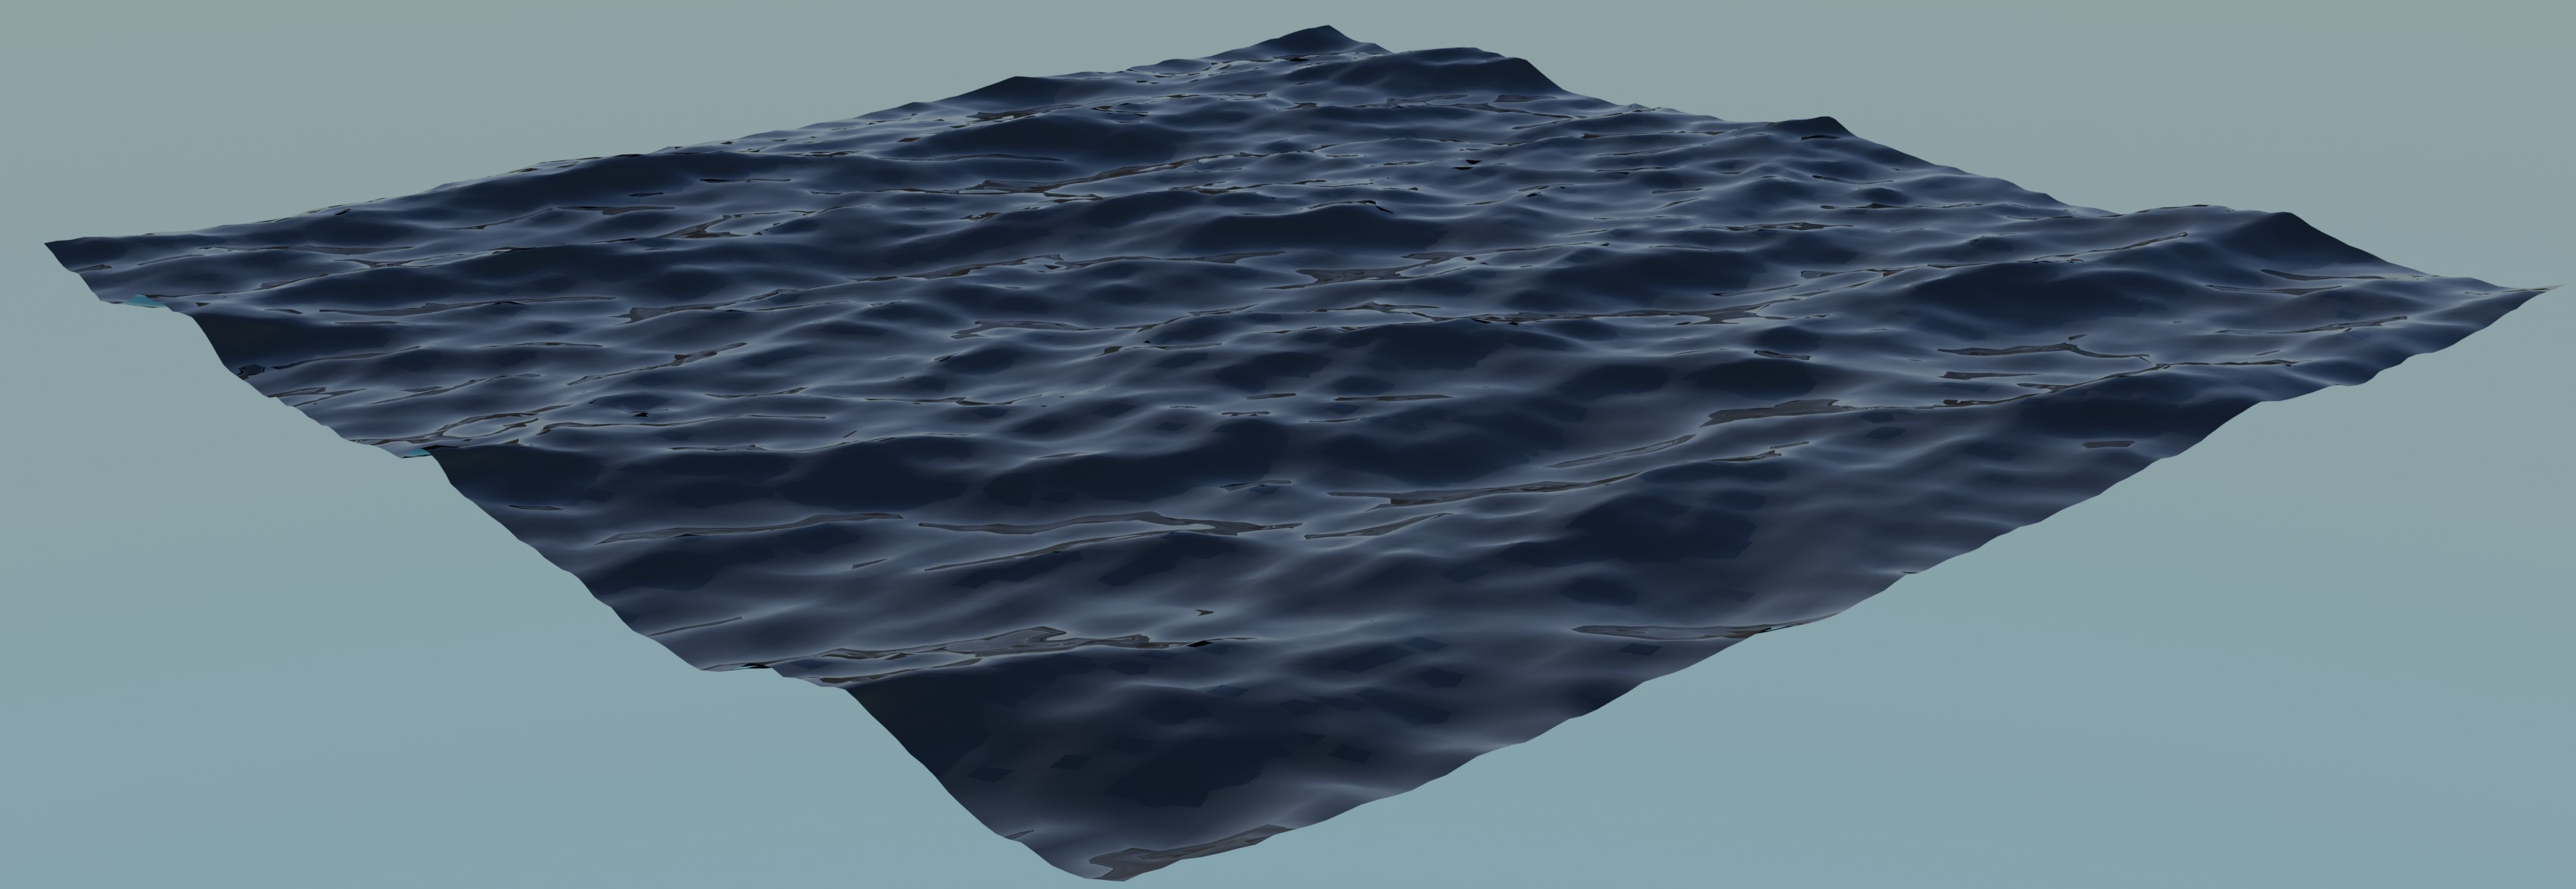
\includegraphics[width=\textwidth]{gfx/prod/ocean/meer0.jpg}
\caption{einzelne Textur als Displacement Map angewendet}
\label{meer0}
\end{figure}

Wenn man nun diese Textur wiederholt zeigen würde, wären Artefakte leicht sichtbar, wie in \autoref{meer1} zu sehen ist.

\begin{figure}[H]
\includegraphics[width=\textwidth]{gfx/prod/ocean/meer1.jpg}
\caption{einzelne Textur gekachelt}
\label{meer1}
\end{figure}

Aus diesem Grund wurden vier unterschiedliche Texturen generiert, welche jeweils zweimal geladen wurden. Diese insgesamt acht Texturen wurden unterschiedlich rotiert skaliert, verschoben, und anschließend übereinander gelegt, damit die nötige Varianz entsteht. Diese problemlos skalierbare Textur ist in \autoref{meer2} zu sehen.

\begin{figure}[H]
\includegraphics[width=\textwidth]{gfx/prod/ocean/meer2.jpg}
\caption{unterschiedliche Texturen gekachelt}
\label{meer2}
\end{figure}

Mit einer zusätzlichen prozeduralen Textur wurde die Intensität der Wellen eingestellt und damit simuliert, dass aufgrund unterschiedlicher Windstärken an unterschiedlichen Orten unterschiedlich starke wellen vorhanden sind. Das Ergebnis der bisherigen Texturen ist in \autoref{meer4} zu sehen.

% \begin{figure}[H]
% \includegraphics[width=\textwidth]{gfx/prod/ocean/meer3.jpg}
% \caption{Meerestextur}
% \label{meer3}
% \end{figure}

\begin{figure}[H]
\includegraphics[width=\textwidth]{gfx/prod/ocean/meer4.jpg}
\caption{Unterschiedliche Intensitäten der Texturen}
\label{meer4}
\end{figure}

Als letzter Part der Wellen wurde noch eine Textur über die bisherigen gelegt. Die in \autoref{meer5} abgebildete Textur stellt das Kielwasser des Segelbootes dar \footfullcite{Wake}. Die Position dieser Textur ist daher auch an die Position des Segelbootes gekoppelt.

\begin{figure}[H]
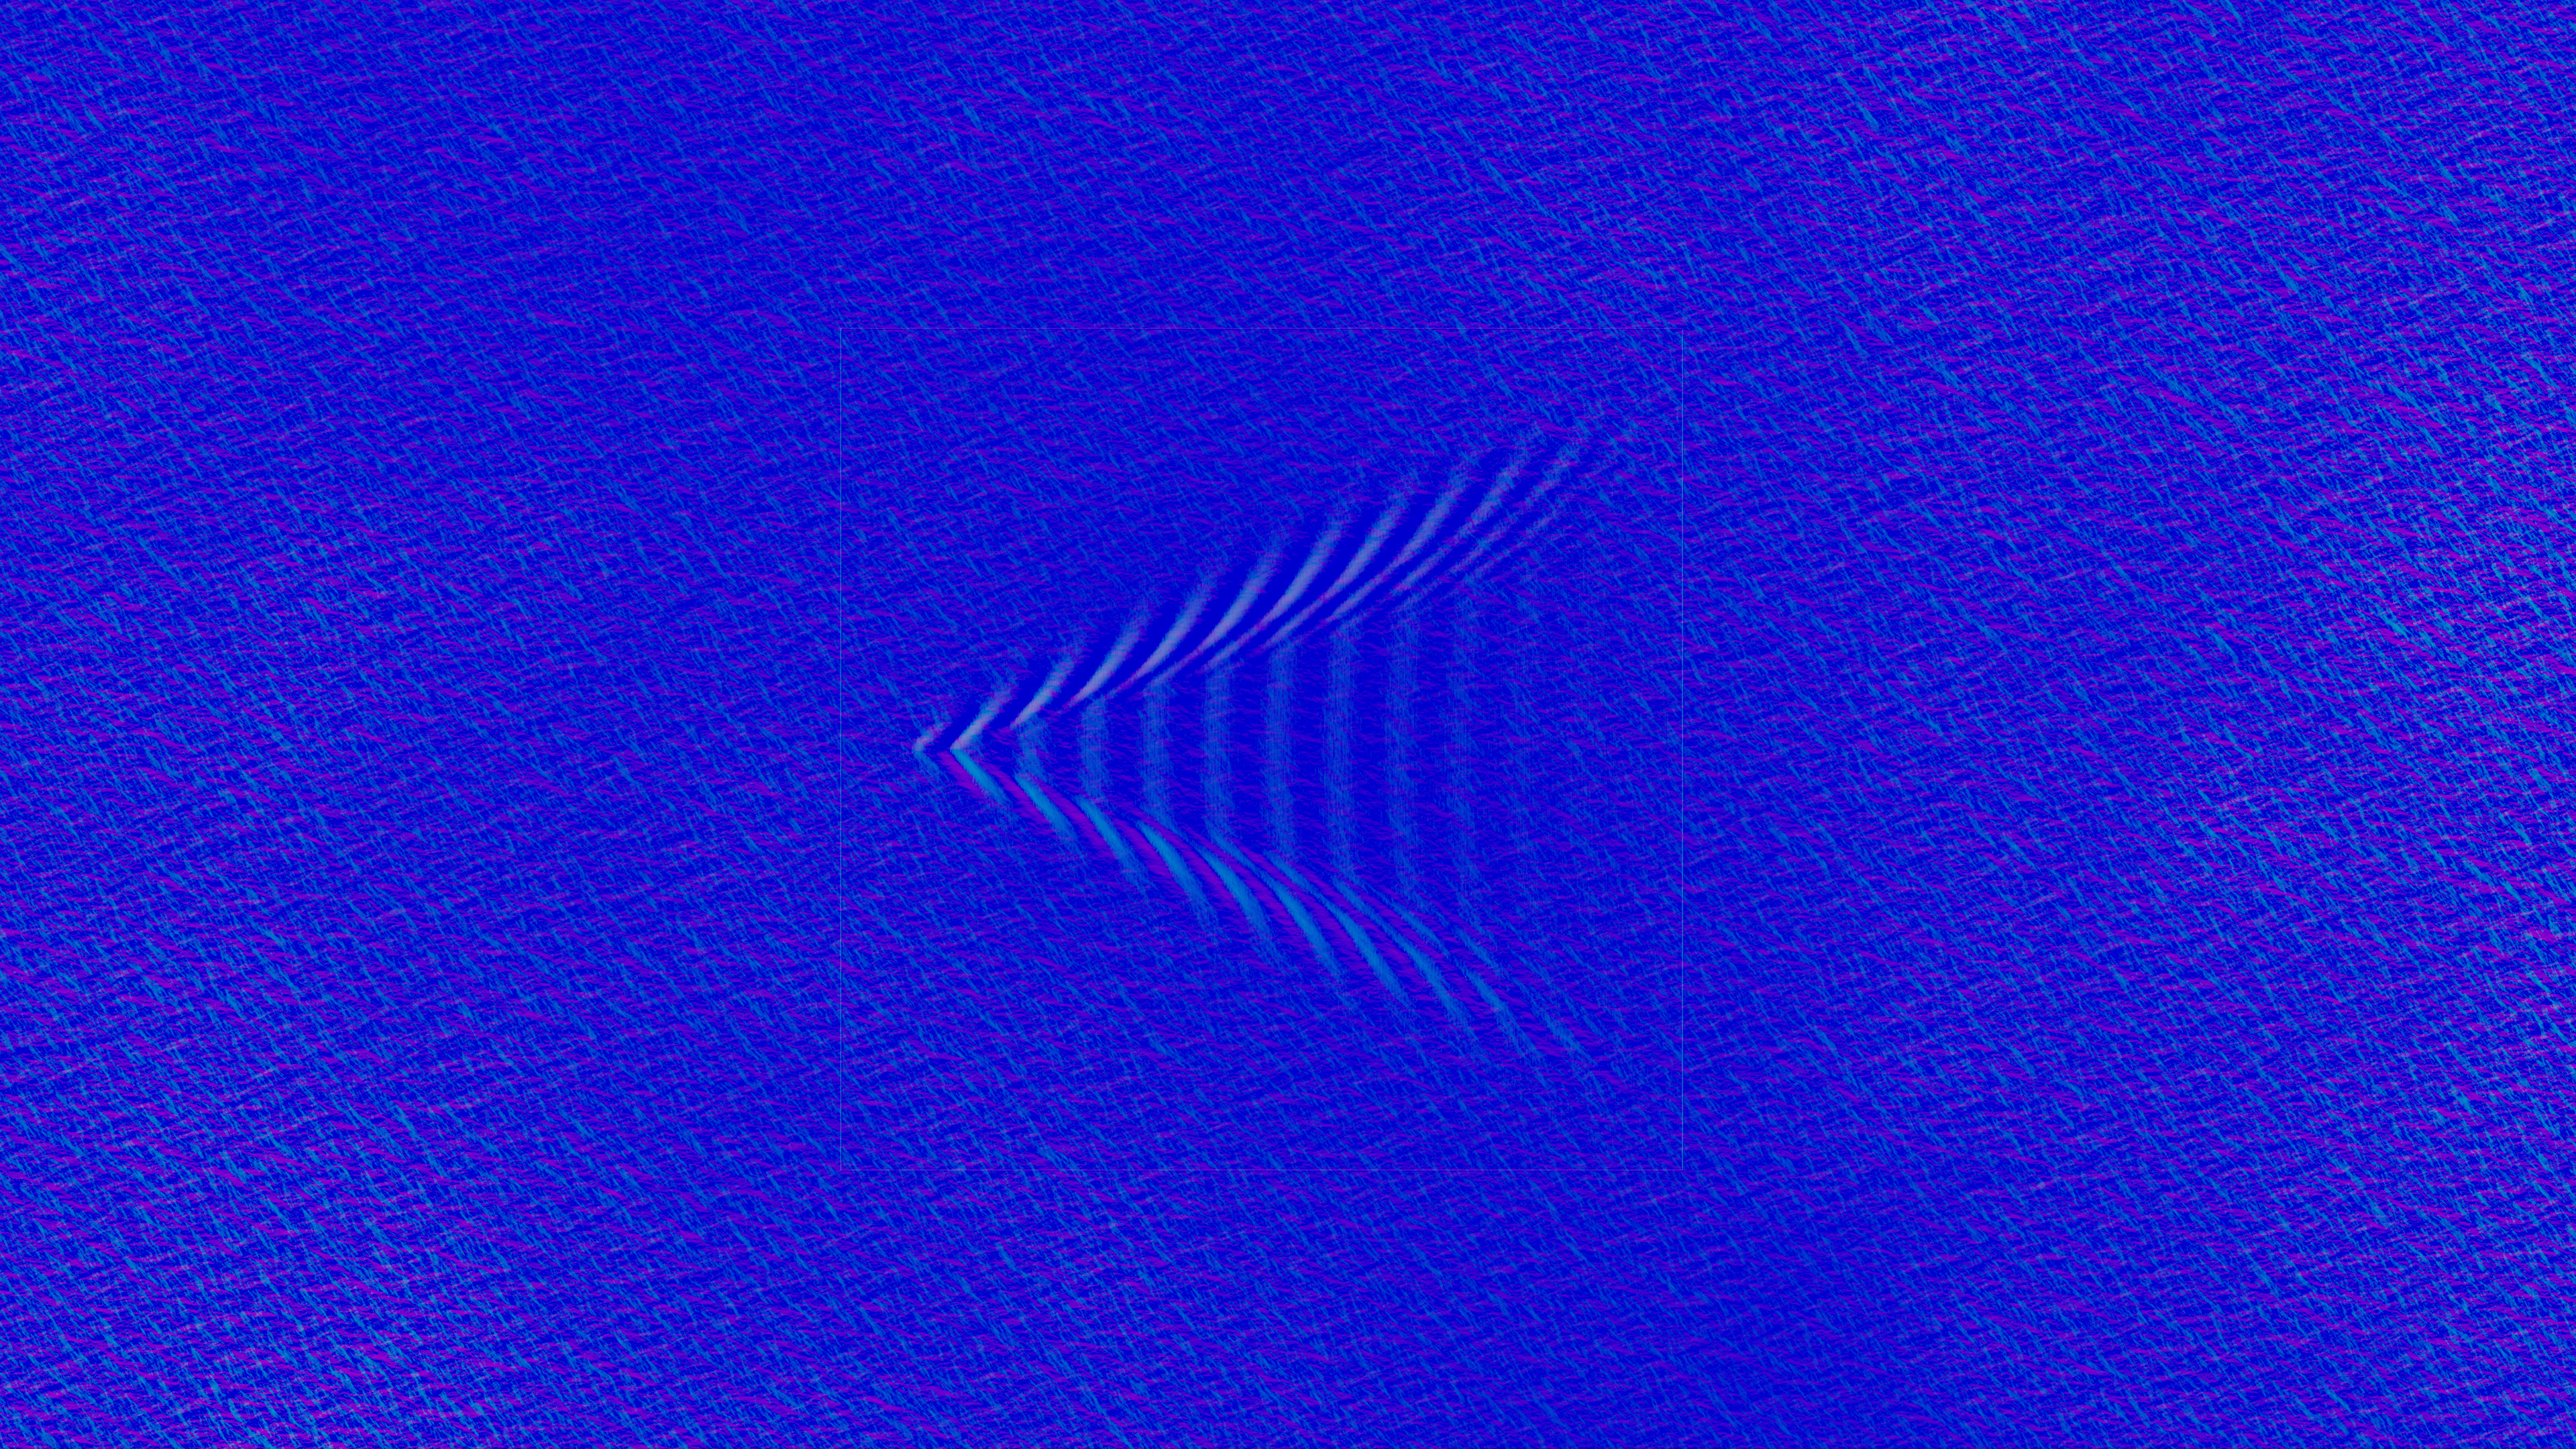
\includegraphics[width=\textwidth]{gfx/prod/ocean/meer5.jpg}
\caption{Kielwasser des Segelbootes als Normal Map}
\label{meer5}
\end{figure}

Weiterhin wurde dem Meer eine leichte farbliche Varianz gegeben, wie in \autoref{meer7} zu sehen ist.

\begin{figure}[H]

\includegraphics[width=\textwidth]{gfx/prod/ocean/meer7.jpg}
\caption{Farbvariationen des Meeres}
\label{meer7}
\end{figure}

In einem weiteren Schritt wurde der Dunst mit einer unüblichen Technik dargestellt. Üblicherweise wird dieser dargestellt, indem mit steigender Entfernung eines Punktes dieser mit der Farbe des Hintergrundes gemischt wird \footfullcite{mist}. Der größere Kreis ist hier Objekt, das das Meer darstellt.\\
Da hier das Meer als einziges Objekt von der Kamera weit entfernt genug war, wurde dieser Effekt direkt im Material abgebildet. Hierbei wird mit einem radialen Gradienten, welcher die Position der Kamera hat, zwischen dem Material des Meeres und einem transparentem Material gemischt. Dieser Gradient ist in \autoref{meer6} sichtbar.

\begin{figure}[H]
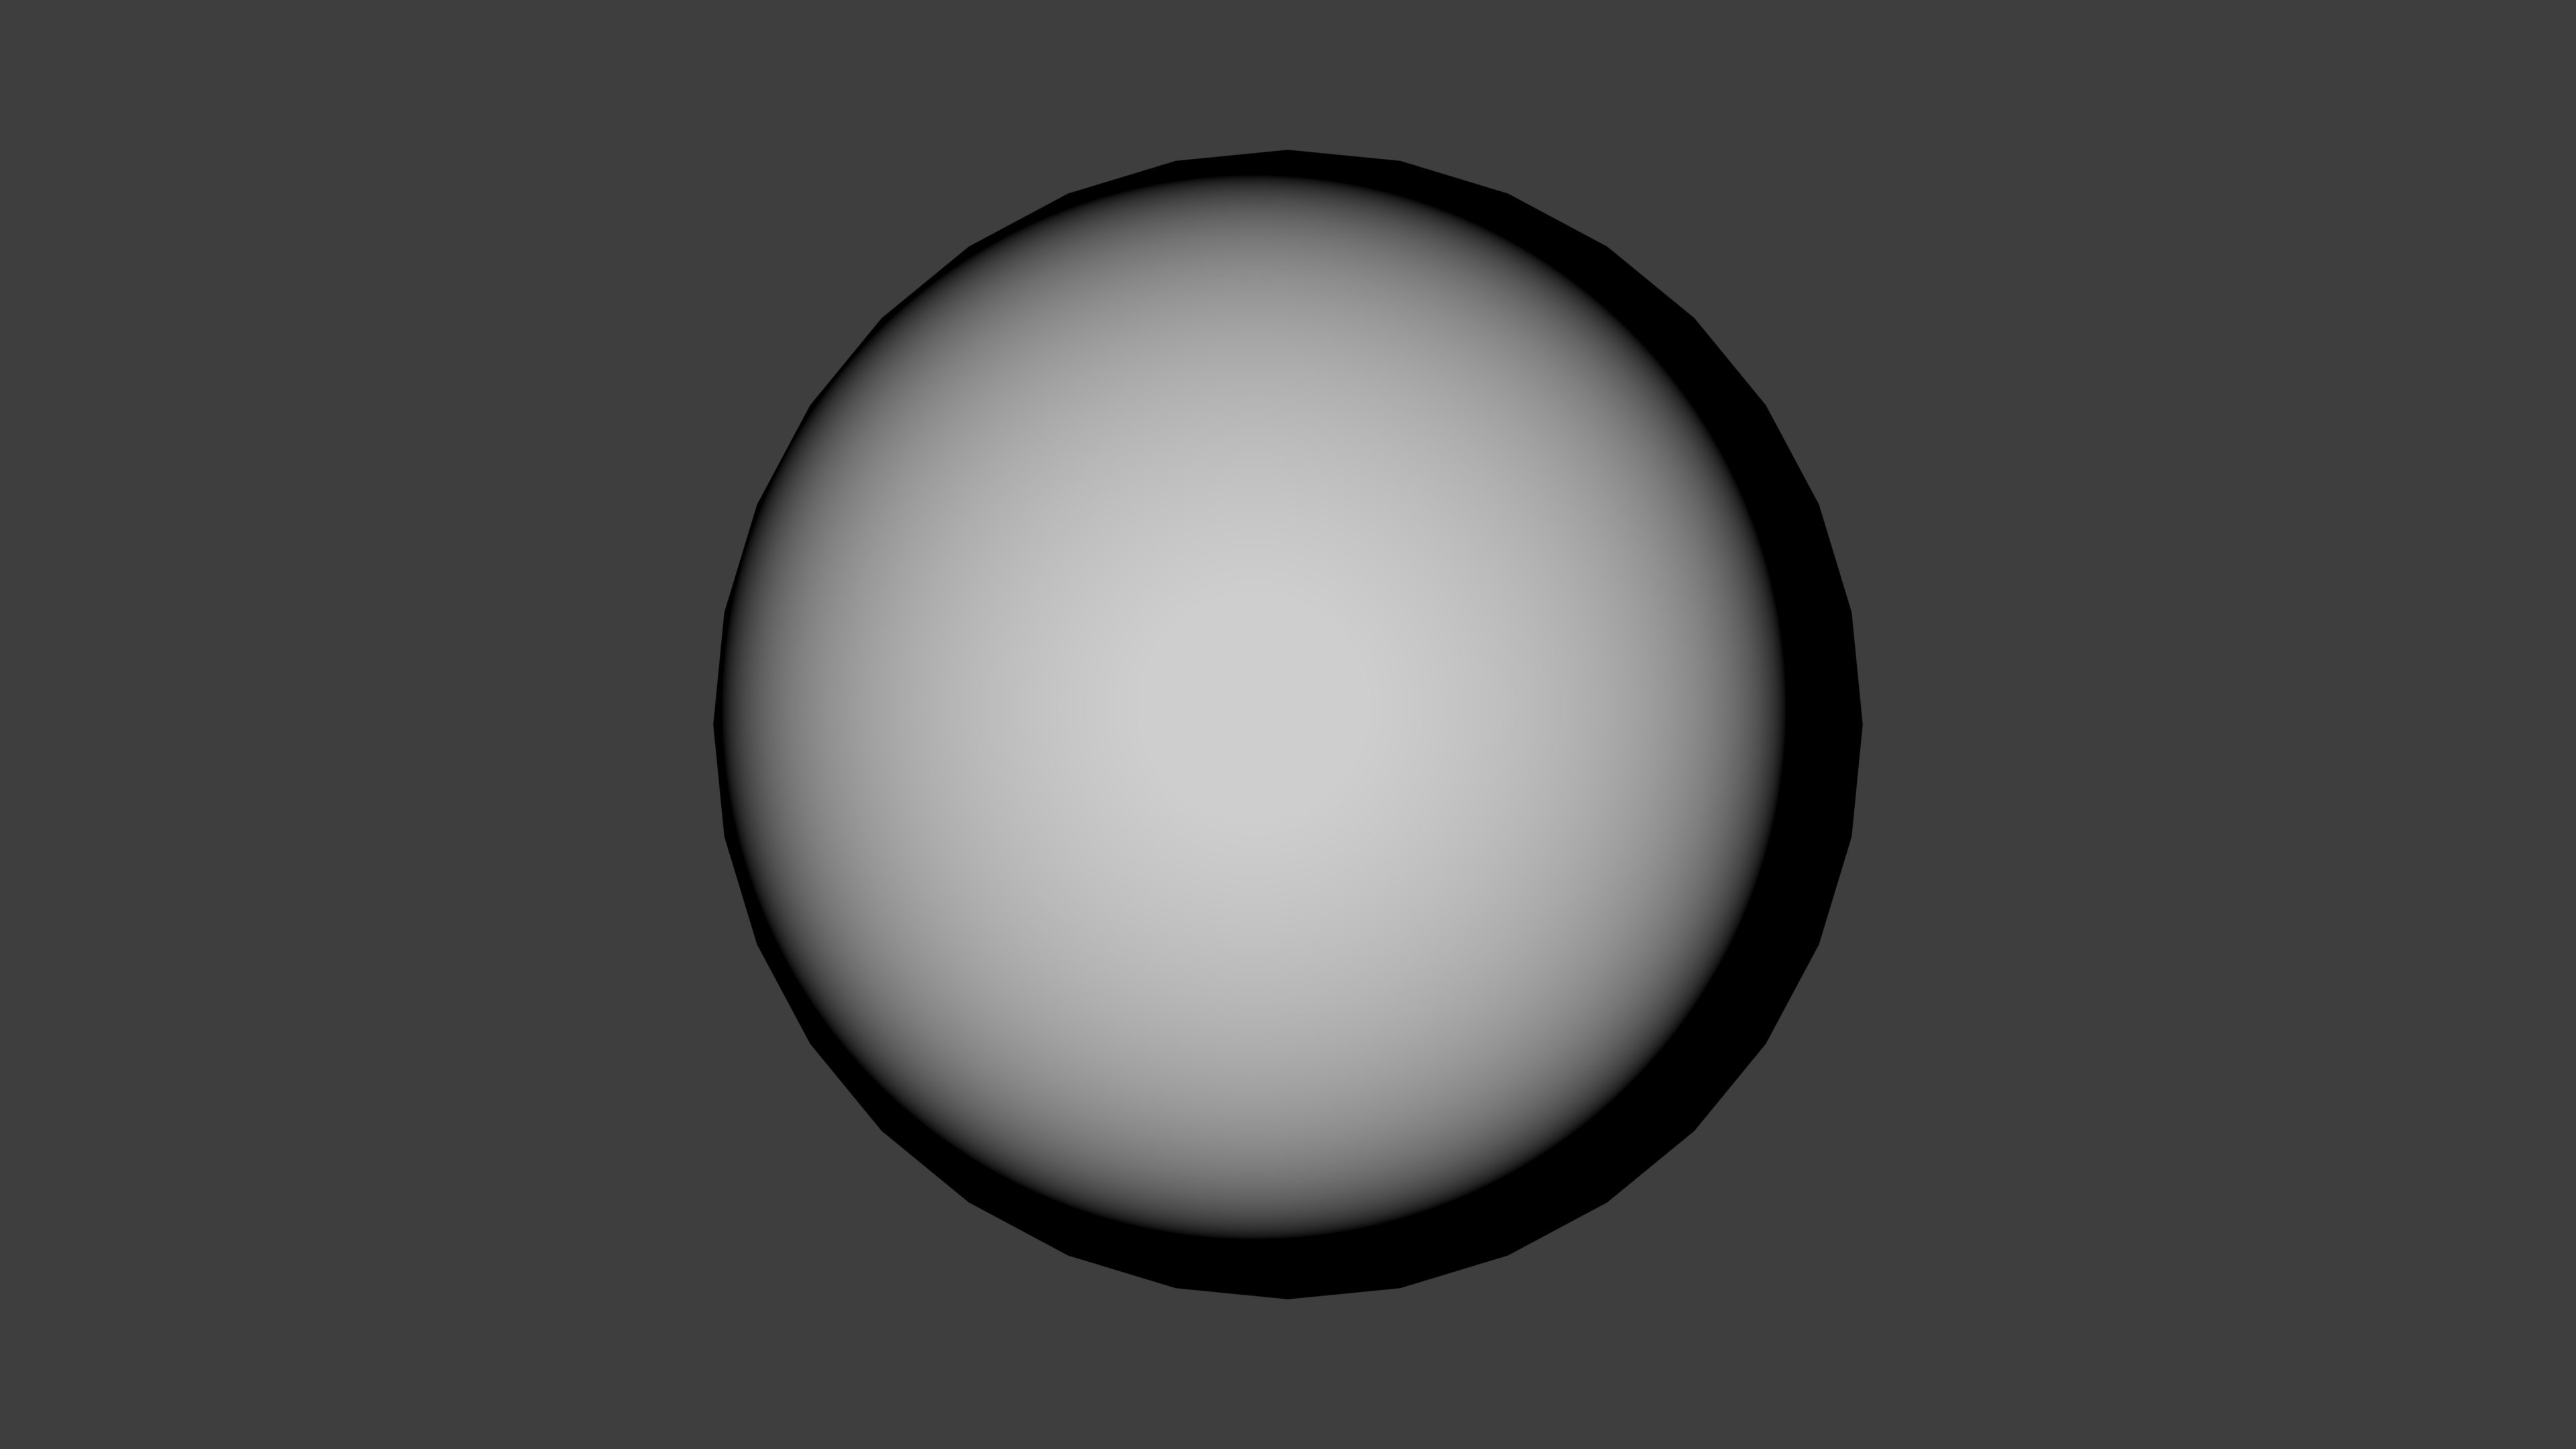
\includegraphics[width=\textwidth]{gfx/prod/ocean/meer6.jpg}
\caption{Gradiententextur für Dunstsimulation}
\label{meer6}
\end{figure}

Der gesamte Aufbau des Materials in Blender.

\begin{figure}[H]
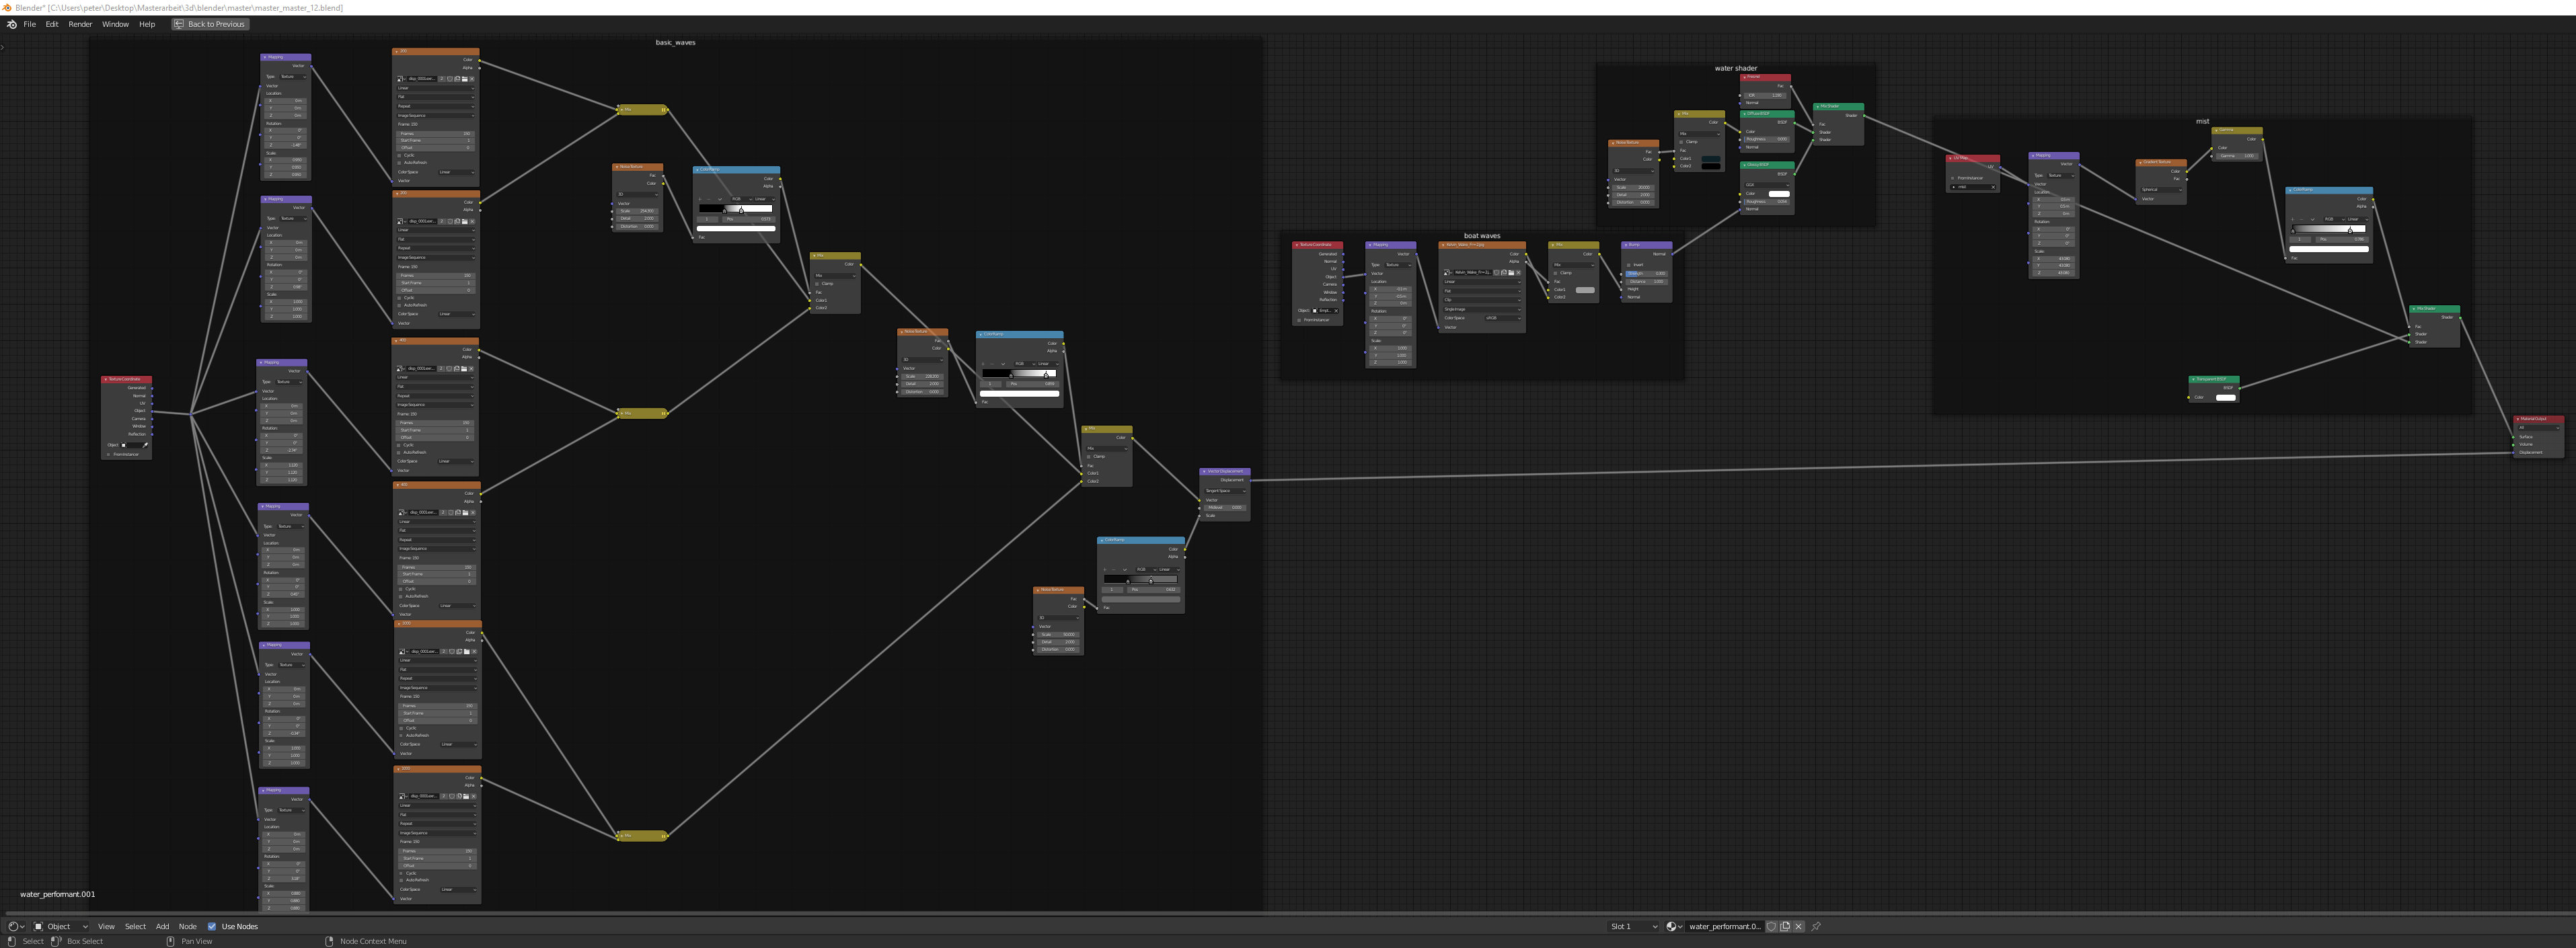
\includegraphics[width=\textwidth]{gfx/prod/env/ocean_shader.jpg}
\caption{Übersicht über den Aufbau des Materials}
\label{ocean_shader}
\end{figure}

\subsection{Himmel}

\begin{figure}[H]
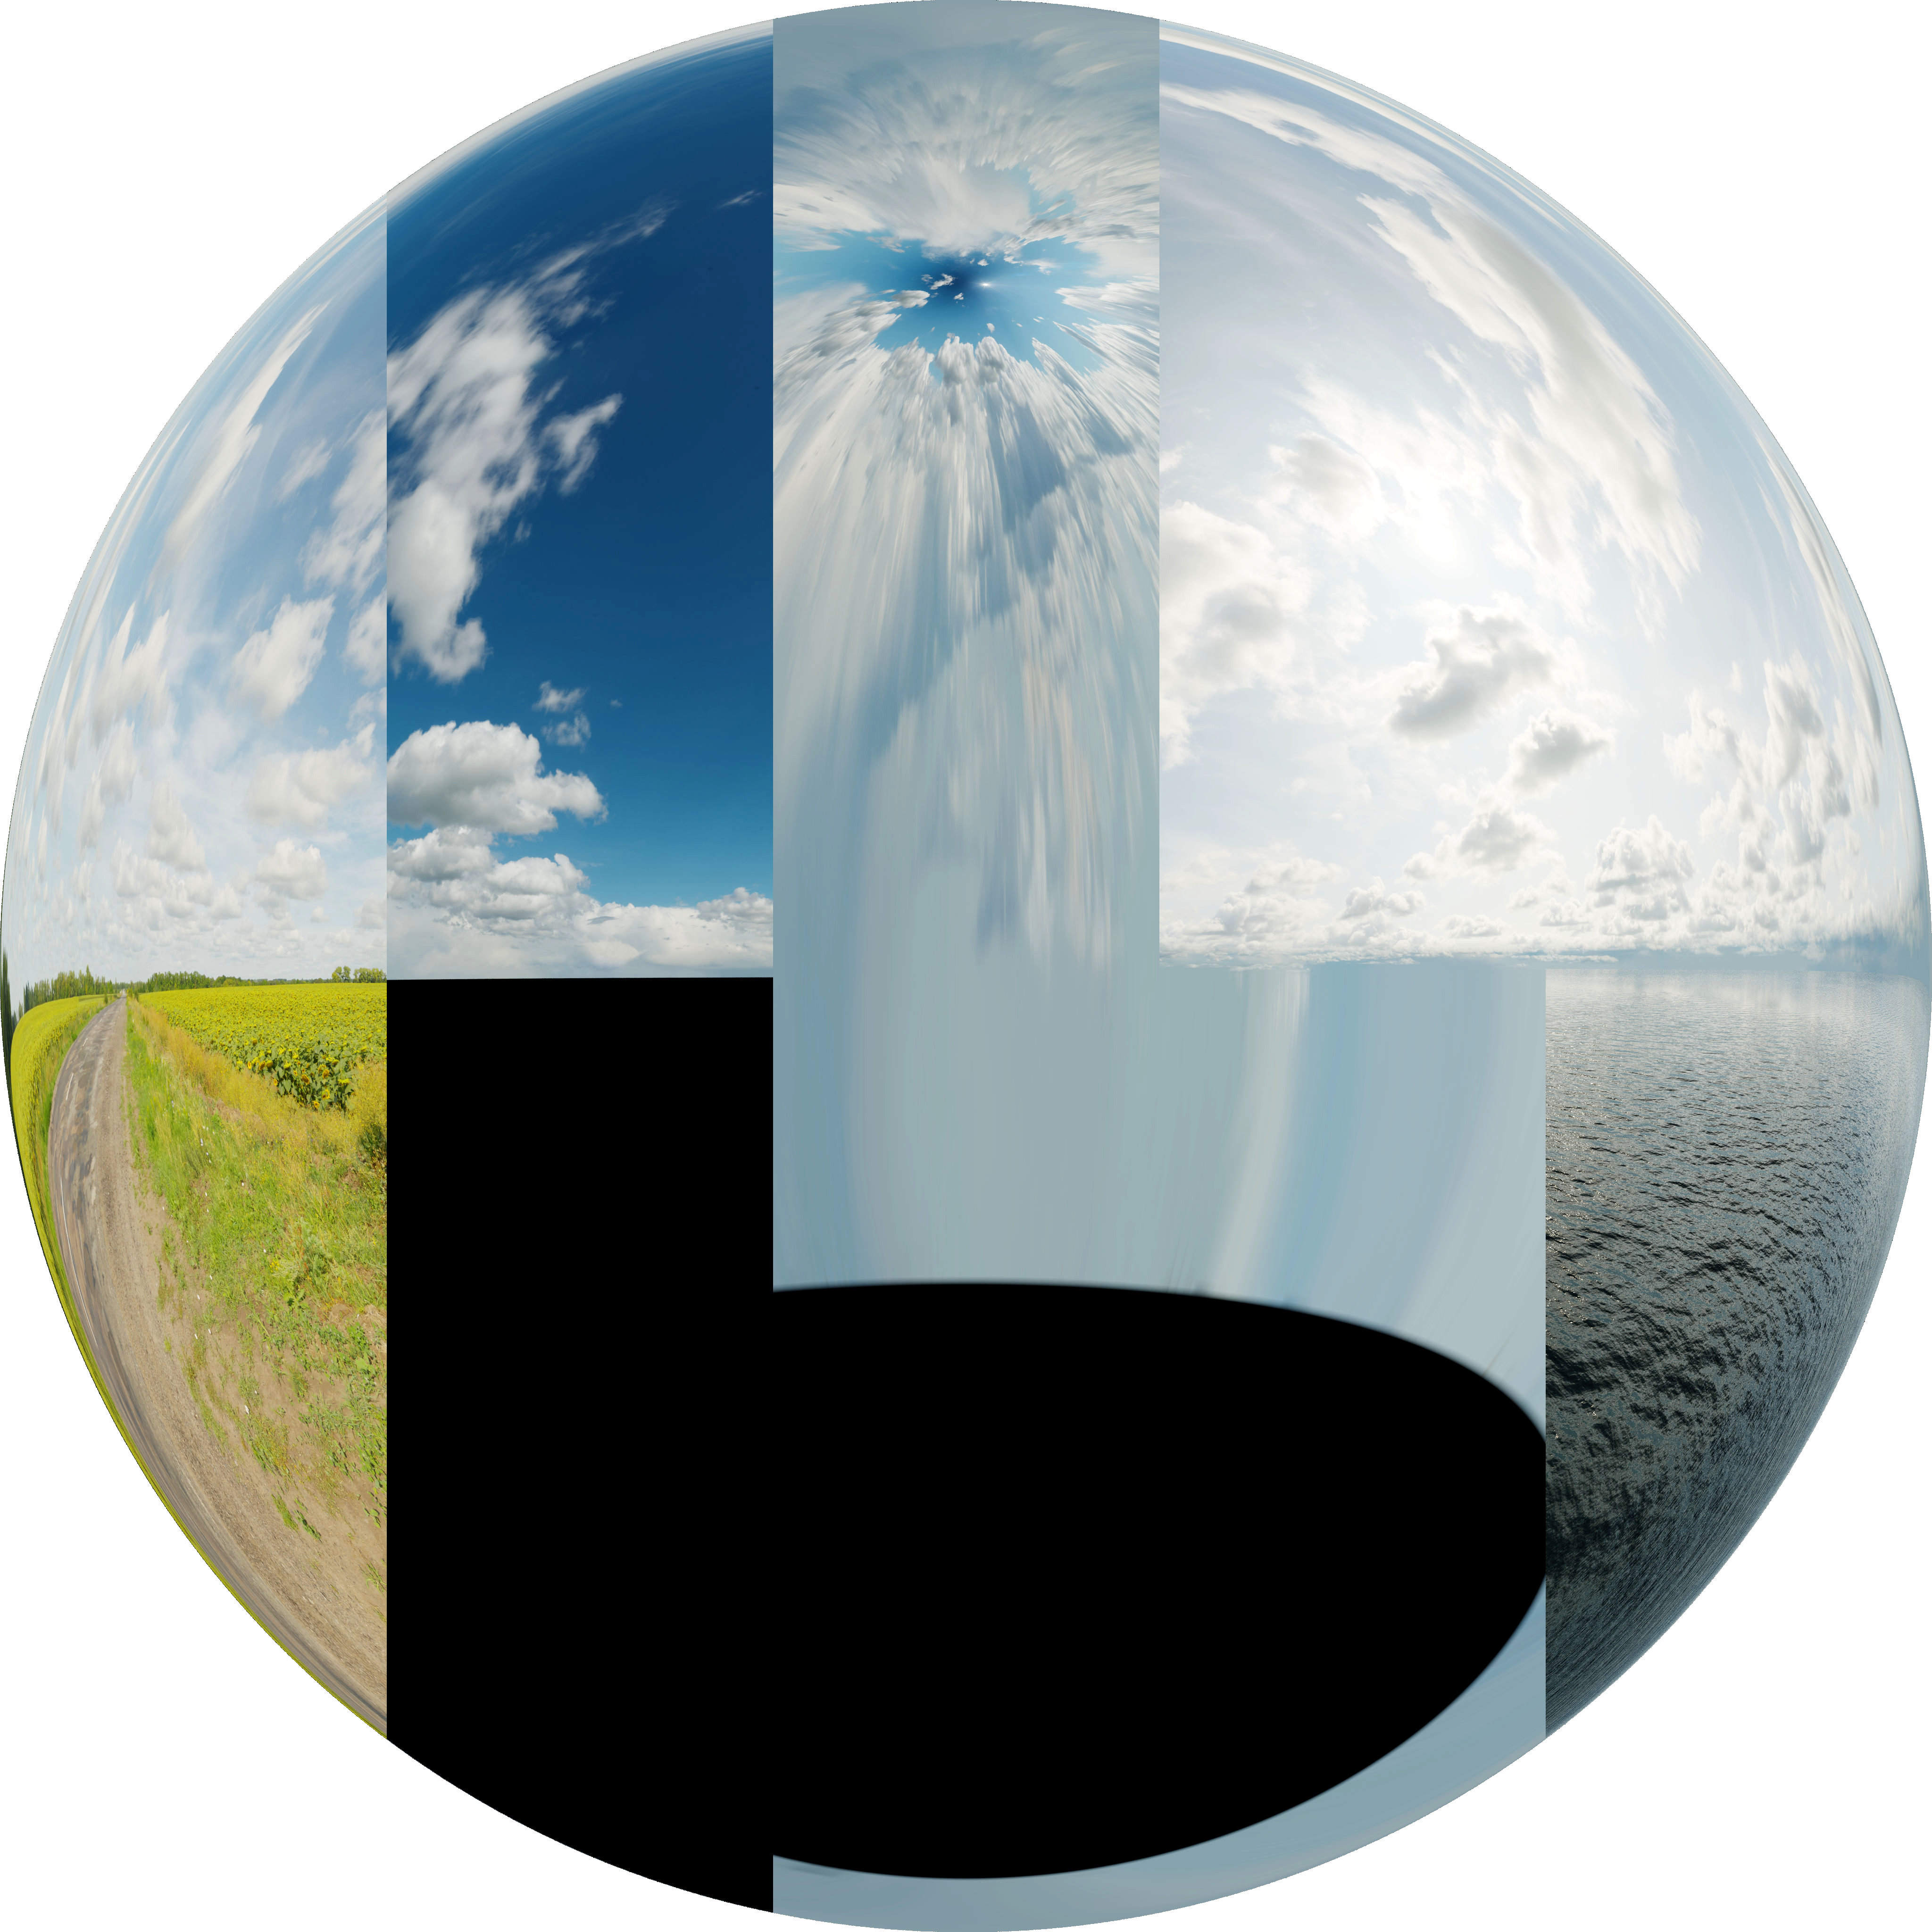
\includegraphics[width=\textwidth]{gfx/prod/env/env.jpg}
\caption{Unterschiedliche Schritte des Himmels}
\label{env}
\end{figure}

Der Hintergrund, bzw. der Himmel war das zweite wichtige Standbein der Umgebung. Zunächst, weil der Himmel ein nicht unwesentlicher Teil des Bildes ist, weil die Optik des Meeres dadurch beeinflusst, dass sich der Himmel darin spiegelt, aber hauptsächlich, weil der Himmel die einzige Lichtquelle in der Szene ist. Die Schwierigkeit bei der Erstellung war, dass die Filmaufnahmen zu unterschiedlichen Zeitpunkten erstellt wurden. Damit musste ein Kompromiss aus Bewölkung und Sonnenstand gemacht werden, damit sich die Computeraufnahmen gut in den Gesamtfilm eingliedern. Die Entscheidung fiel hierbei auf die Textur links in \autoref{env} \footfullcite{Sunflowers}. Diese Textur hat eine sehr hohe Qualität und passt ebenfalls sehr gut zum Filmmaterial. Nachteil der Textur war, dass einige Bäume über dem Horizont noch sichtbar sind. Deswegen wurde im Bereich des Horizontes eine andere Textur \footfullcite{Sky}, die grundsätzlich nicht so gut zum Filmmaterial passt, verwendet (siehe \autoref{env}, zweite Spalte).\\
Durch die vergleichsweise hohe Flughöhe der Drohne, sieht man jedoch etwas tiefer als der Horizont in der Textur geht. Dies hatte zur Folge, dass der schwarze Bereich sichtbar war. Dies wurde umgangen, indem hier anstatt des schwarzen Bereiches eine vertikal skalierte Version gezeigt wurde (siehe dritte Spalte).\\
Diese drei Texturen bilden abschließend den fertigen Himmel, wie in der vierten Spalte zu sehen ist. In der fünften und letzten Spalte ist als Vergleich das Meer zusätzlich eingefügt.

\subsection{Segelboot}

% \begin{wrapfigure}{r}{0.5\textwidth}
% \begin{center}
% 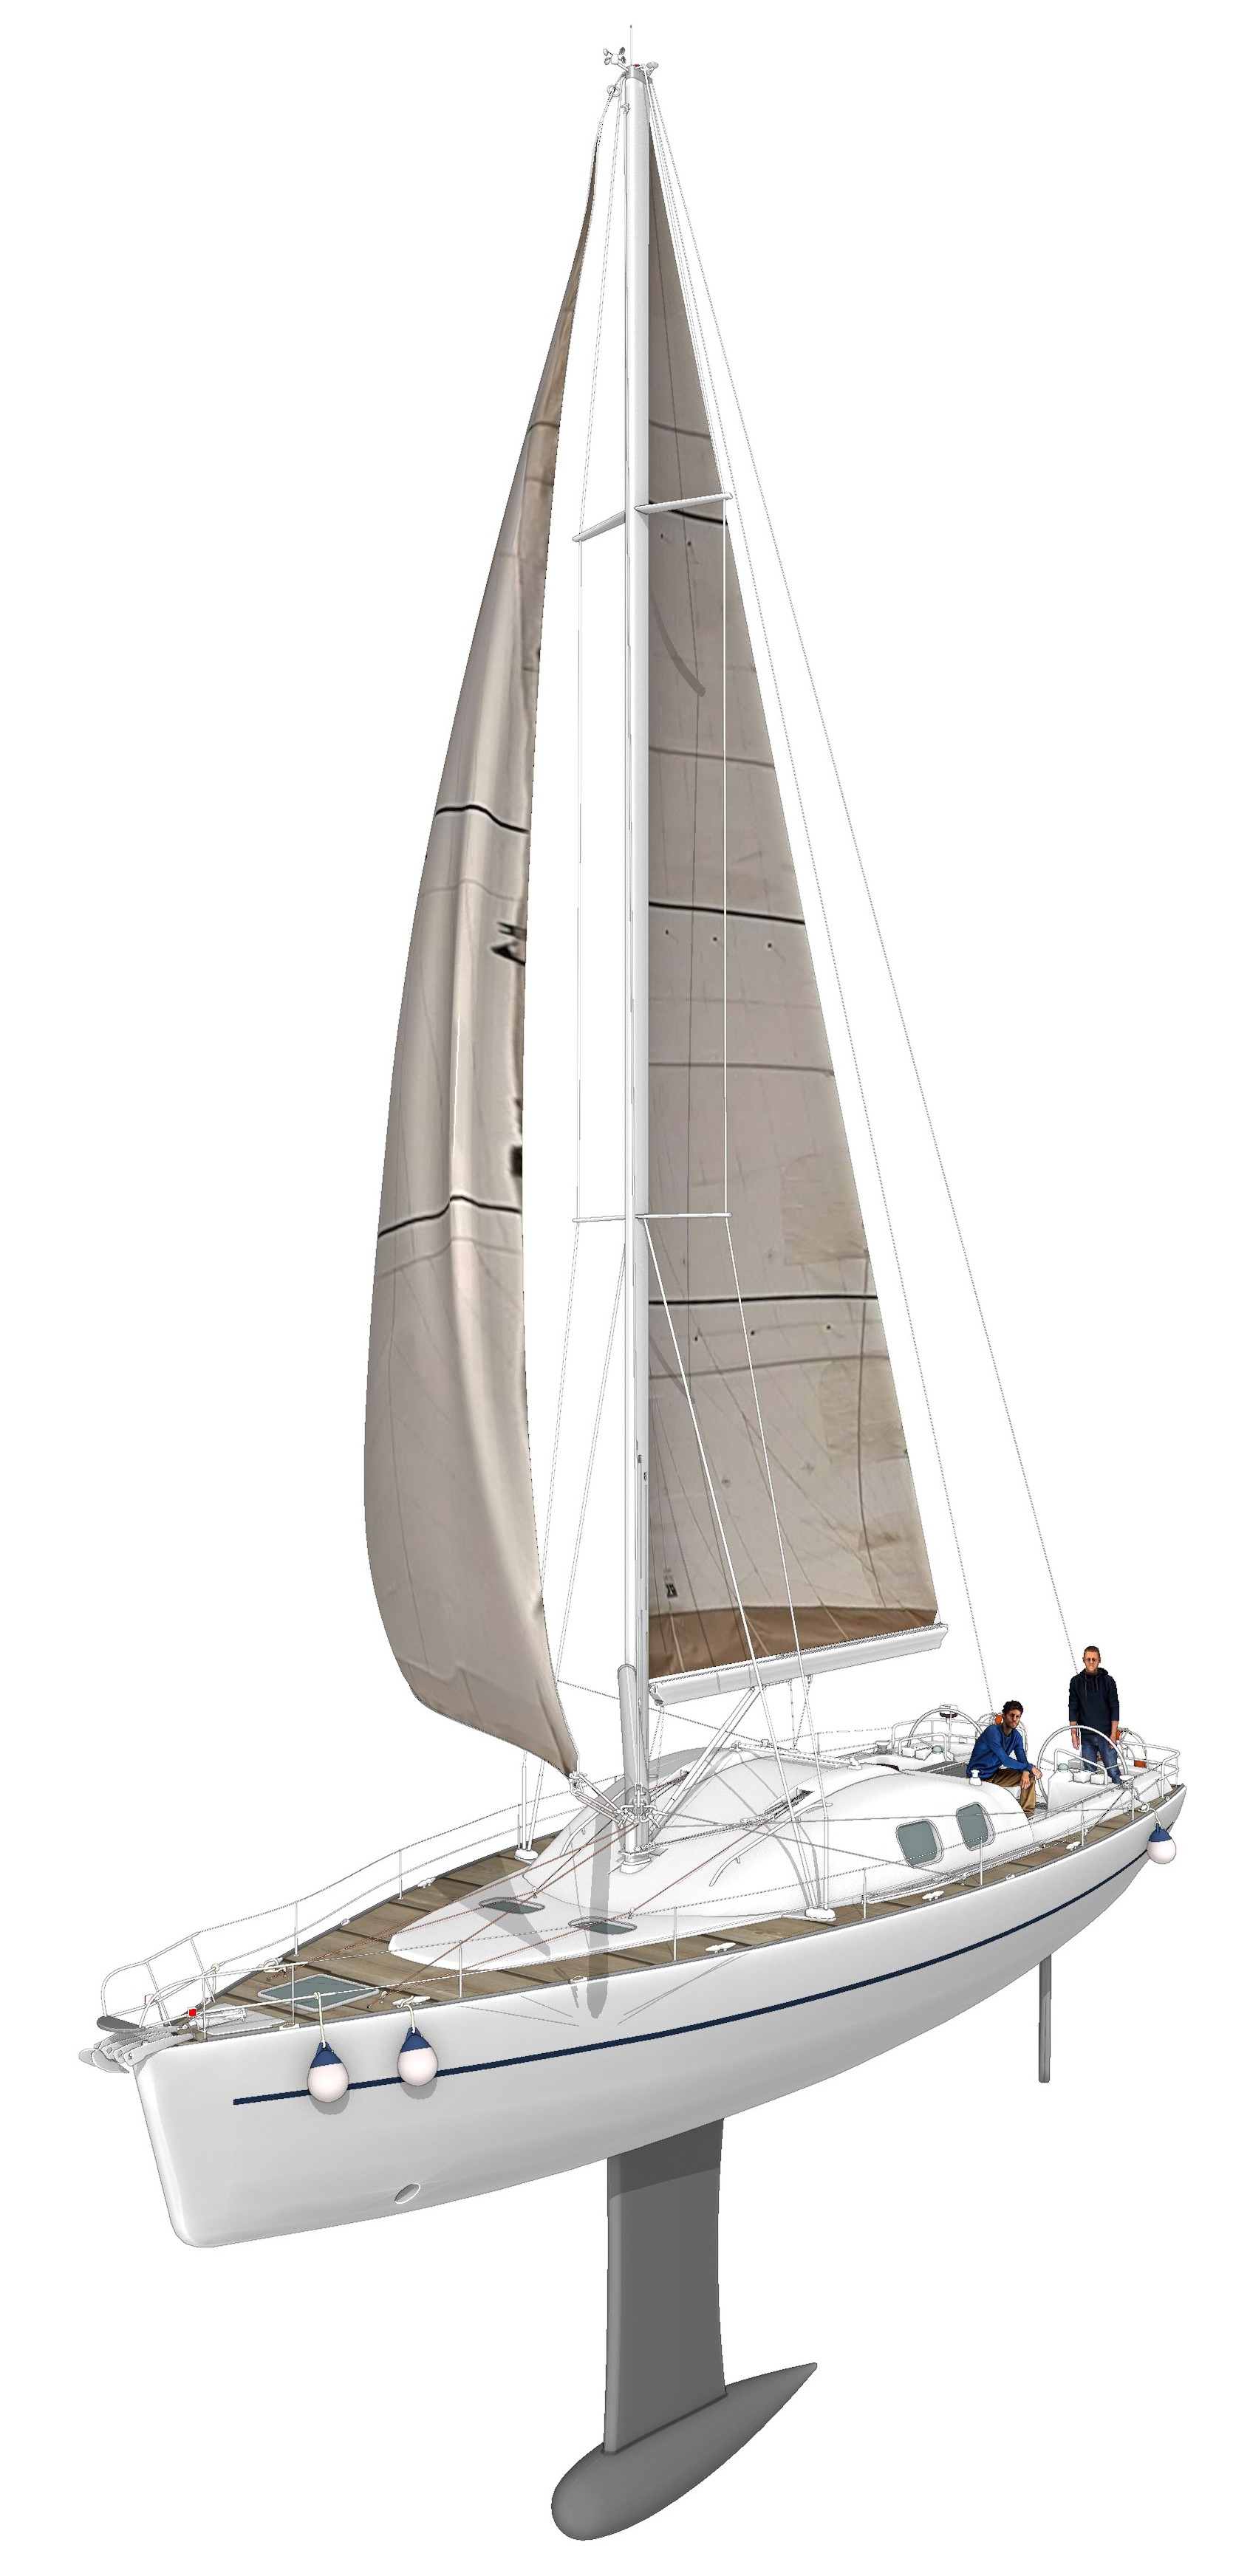
\includegraphics[width=0.2\textwidth]{gfx/prod/boat/boat.jpg}
% \end{center}
% \caption{Segelboot mit Materialien}
% \label{segelboot_modell}
% \end{wrapfigure}

\begin{figure}[H]
\begin{center}
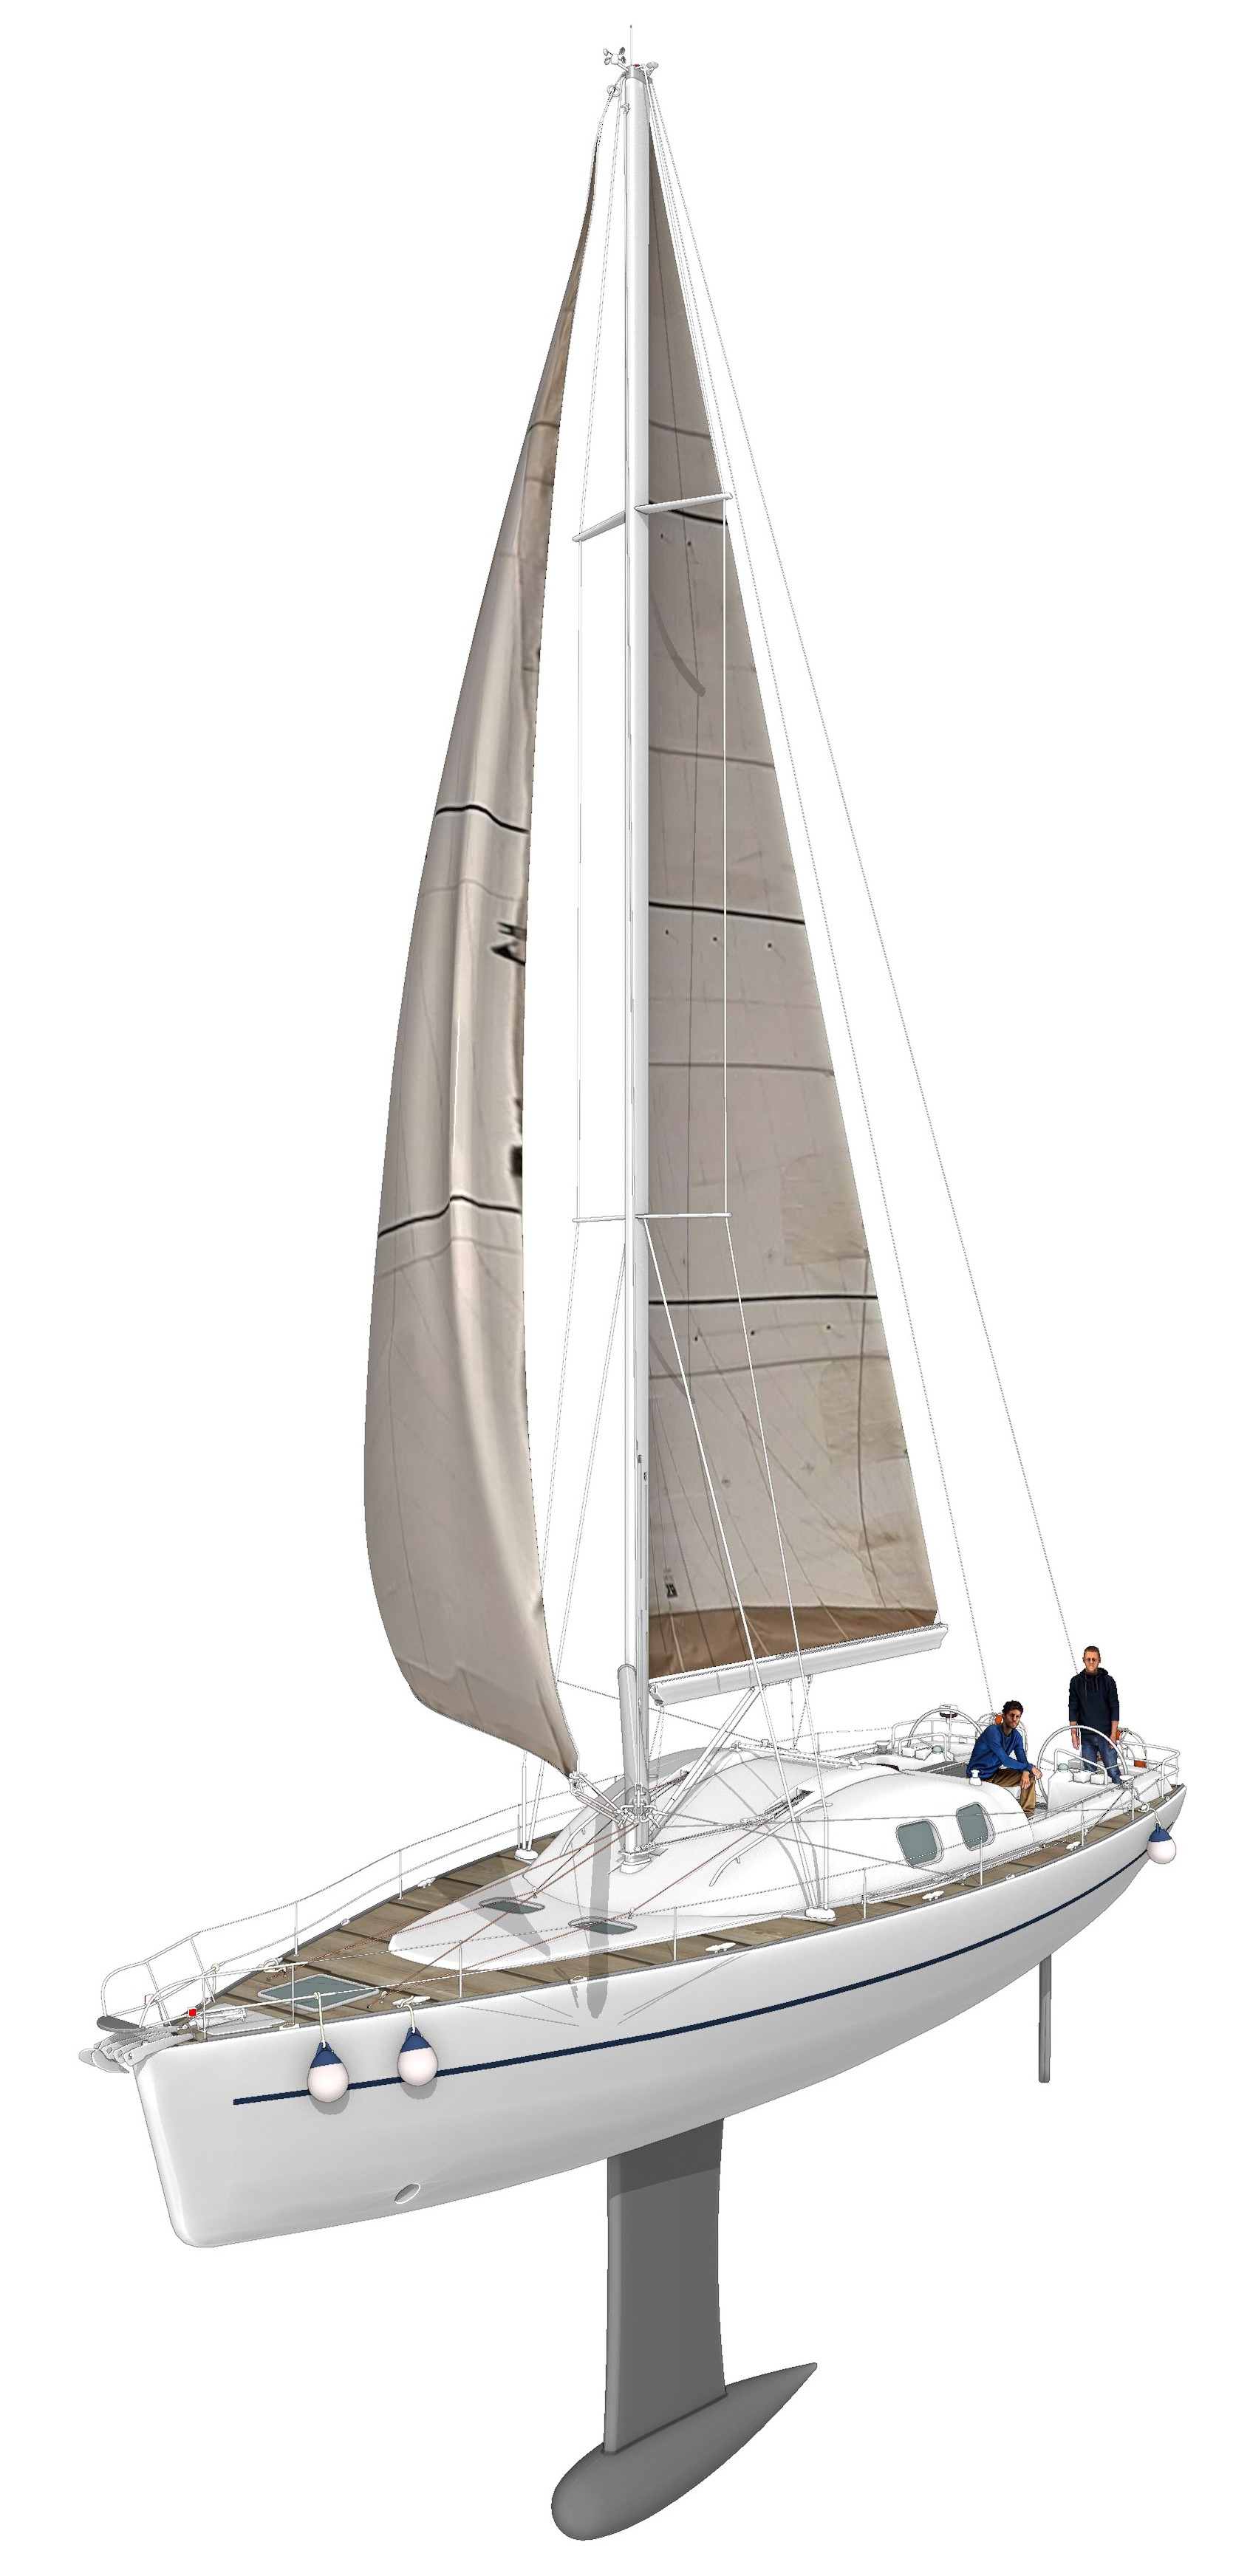
\includegraphics[width=0.5\textwidth]{gfx/prod/boat/boat.jpg}
\end{center}
\caption{Segelboot mit Materialien}
\label{segelboot_modell}
\end{figure}

Das heruntergeladene CAD-Modell des Segelbootes wurde in Blender importiert und mit passenden Materialien versehen \footfullcite{Sailboat}. Auf das Segel wurde ein Bild eines Segelbootes projiziert, damit die Struktur und die Nähte sichtbar sind \footfullcite{impression}. Anschließend wurden zwei Modelle von Menschen hinzugefügt \footfullcite{people}. Das Ergebnis des Bootes ist in \autoref{segelboot_modell} abgebildet.

\section{Drohne}

\subsection{Modellierung}

Als Grundlage für das Modell der Drohne hat ein Fotoscan gedient. Hierzu wurden mit einem Smartphone etwa 250 Fotos der Drohne für zwei Scans angefertigt -- einmal von oben und einmal von unten. Anschließend wurden die Bilder in die Fotoscansoftware Meshroom geladen und zu einem texturierten 3D-Modell gewandelt. Dieser Vorgang ist in \autoref{meshroom1} und \autoref{meshroom2} dargestellt. Leider wurden von der Seite des Modells nicht ausreichend Bilder erstellt, sodass teilweise ein Spalt vorhanden war, wie in \autoref{drohne_modell} zu sehen ist.\\
\begin{figure}[H]
\begin{center}
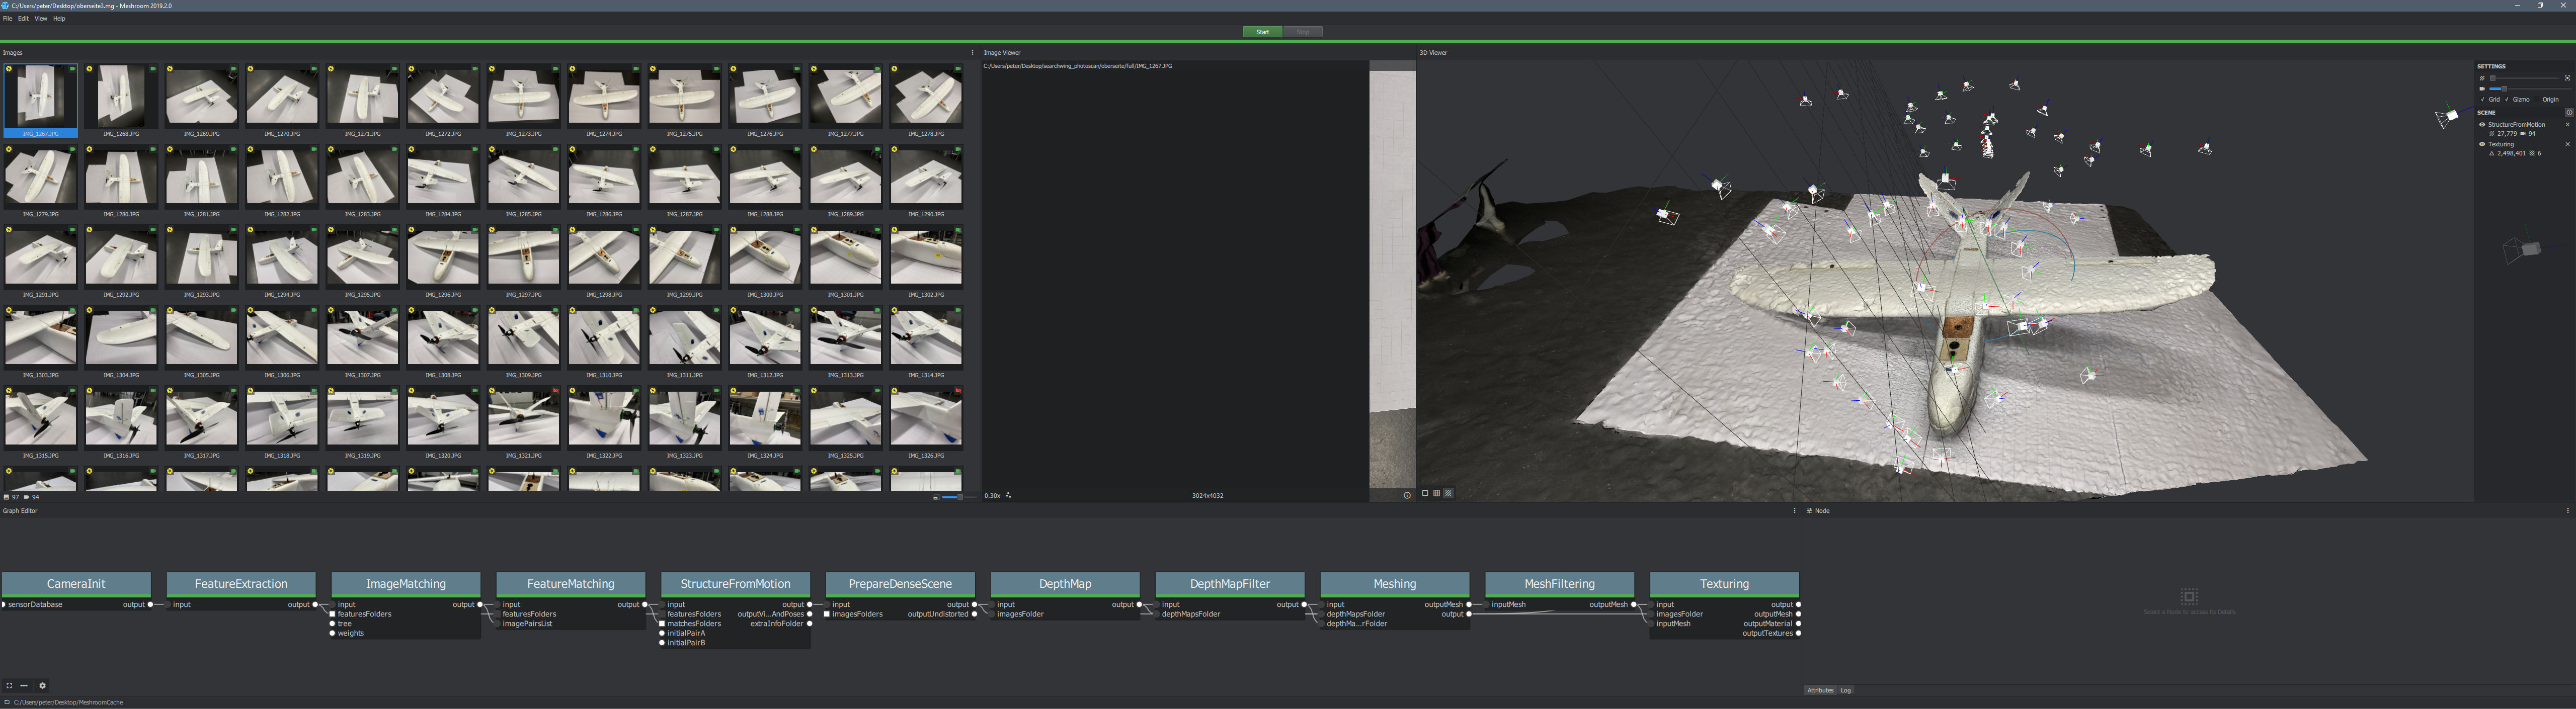
\includegraphics[width=\textwidth]{gfx/prod/plane/meshroom1.jpg}
\caption{Fotoscan in Meshroom, Drohne von oben}
\label{meshroom1}
\end{center}
\end{figure}

\begin{figure}[H]
\begin{center}
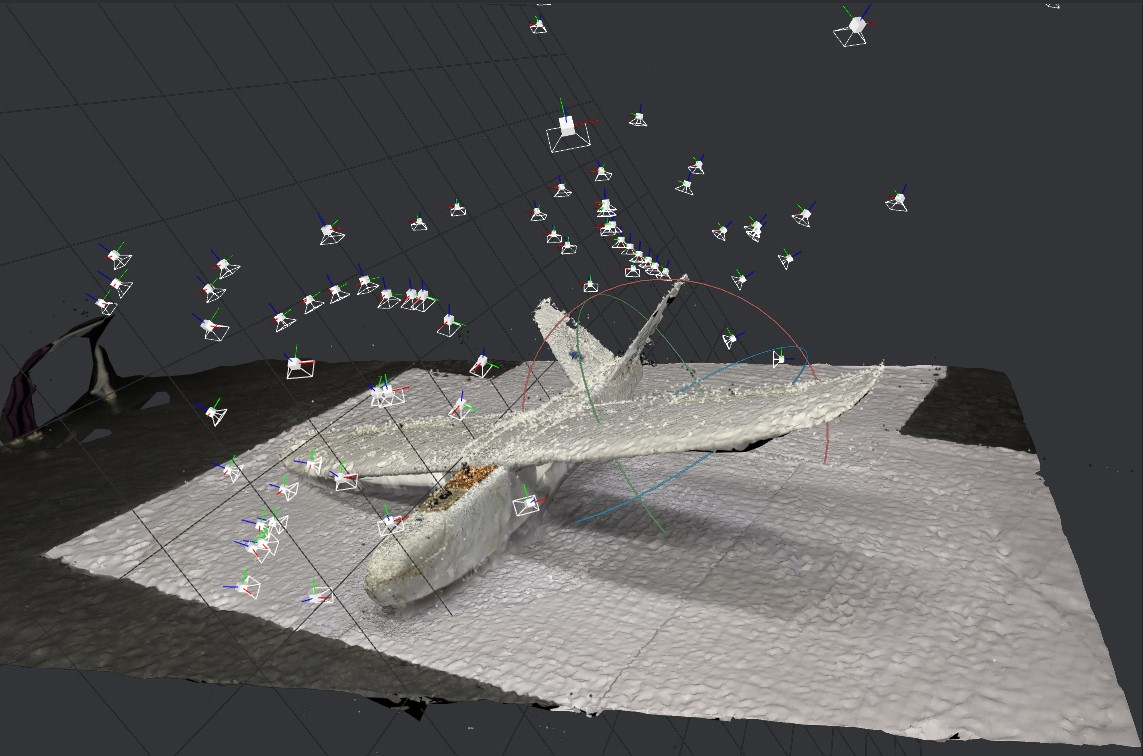
\includegraphics[width=\textwidth]{gfx/prod/plane/meshroom2.jpg}
\caption{Fotoscan in Meshroom, Drohne von unten}
\label{meshroom2}
\end{center}
\end{figure}

Für den Rumpf wurde ein CAD-Modell bereitgestellt, der nur leicht nachbearbeitet werden musste. Flügel und Leitwerke wurden selbst modelliert.\\
Die übrigen Kleinteile, wie Servomotoren \footfullcite{Hobby}, Propeller \footfullcite{propeller}, Elektromotor \footfullcite{brushless} und Schalter \footfullcite{Rocker} wurden ebenfalls als CAD-Daten importiert, und anschließend mit Materialien versehen.

\begin{figure}[H]
\begin{center}
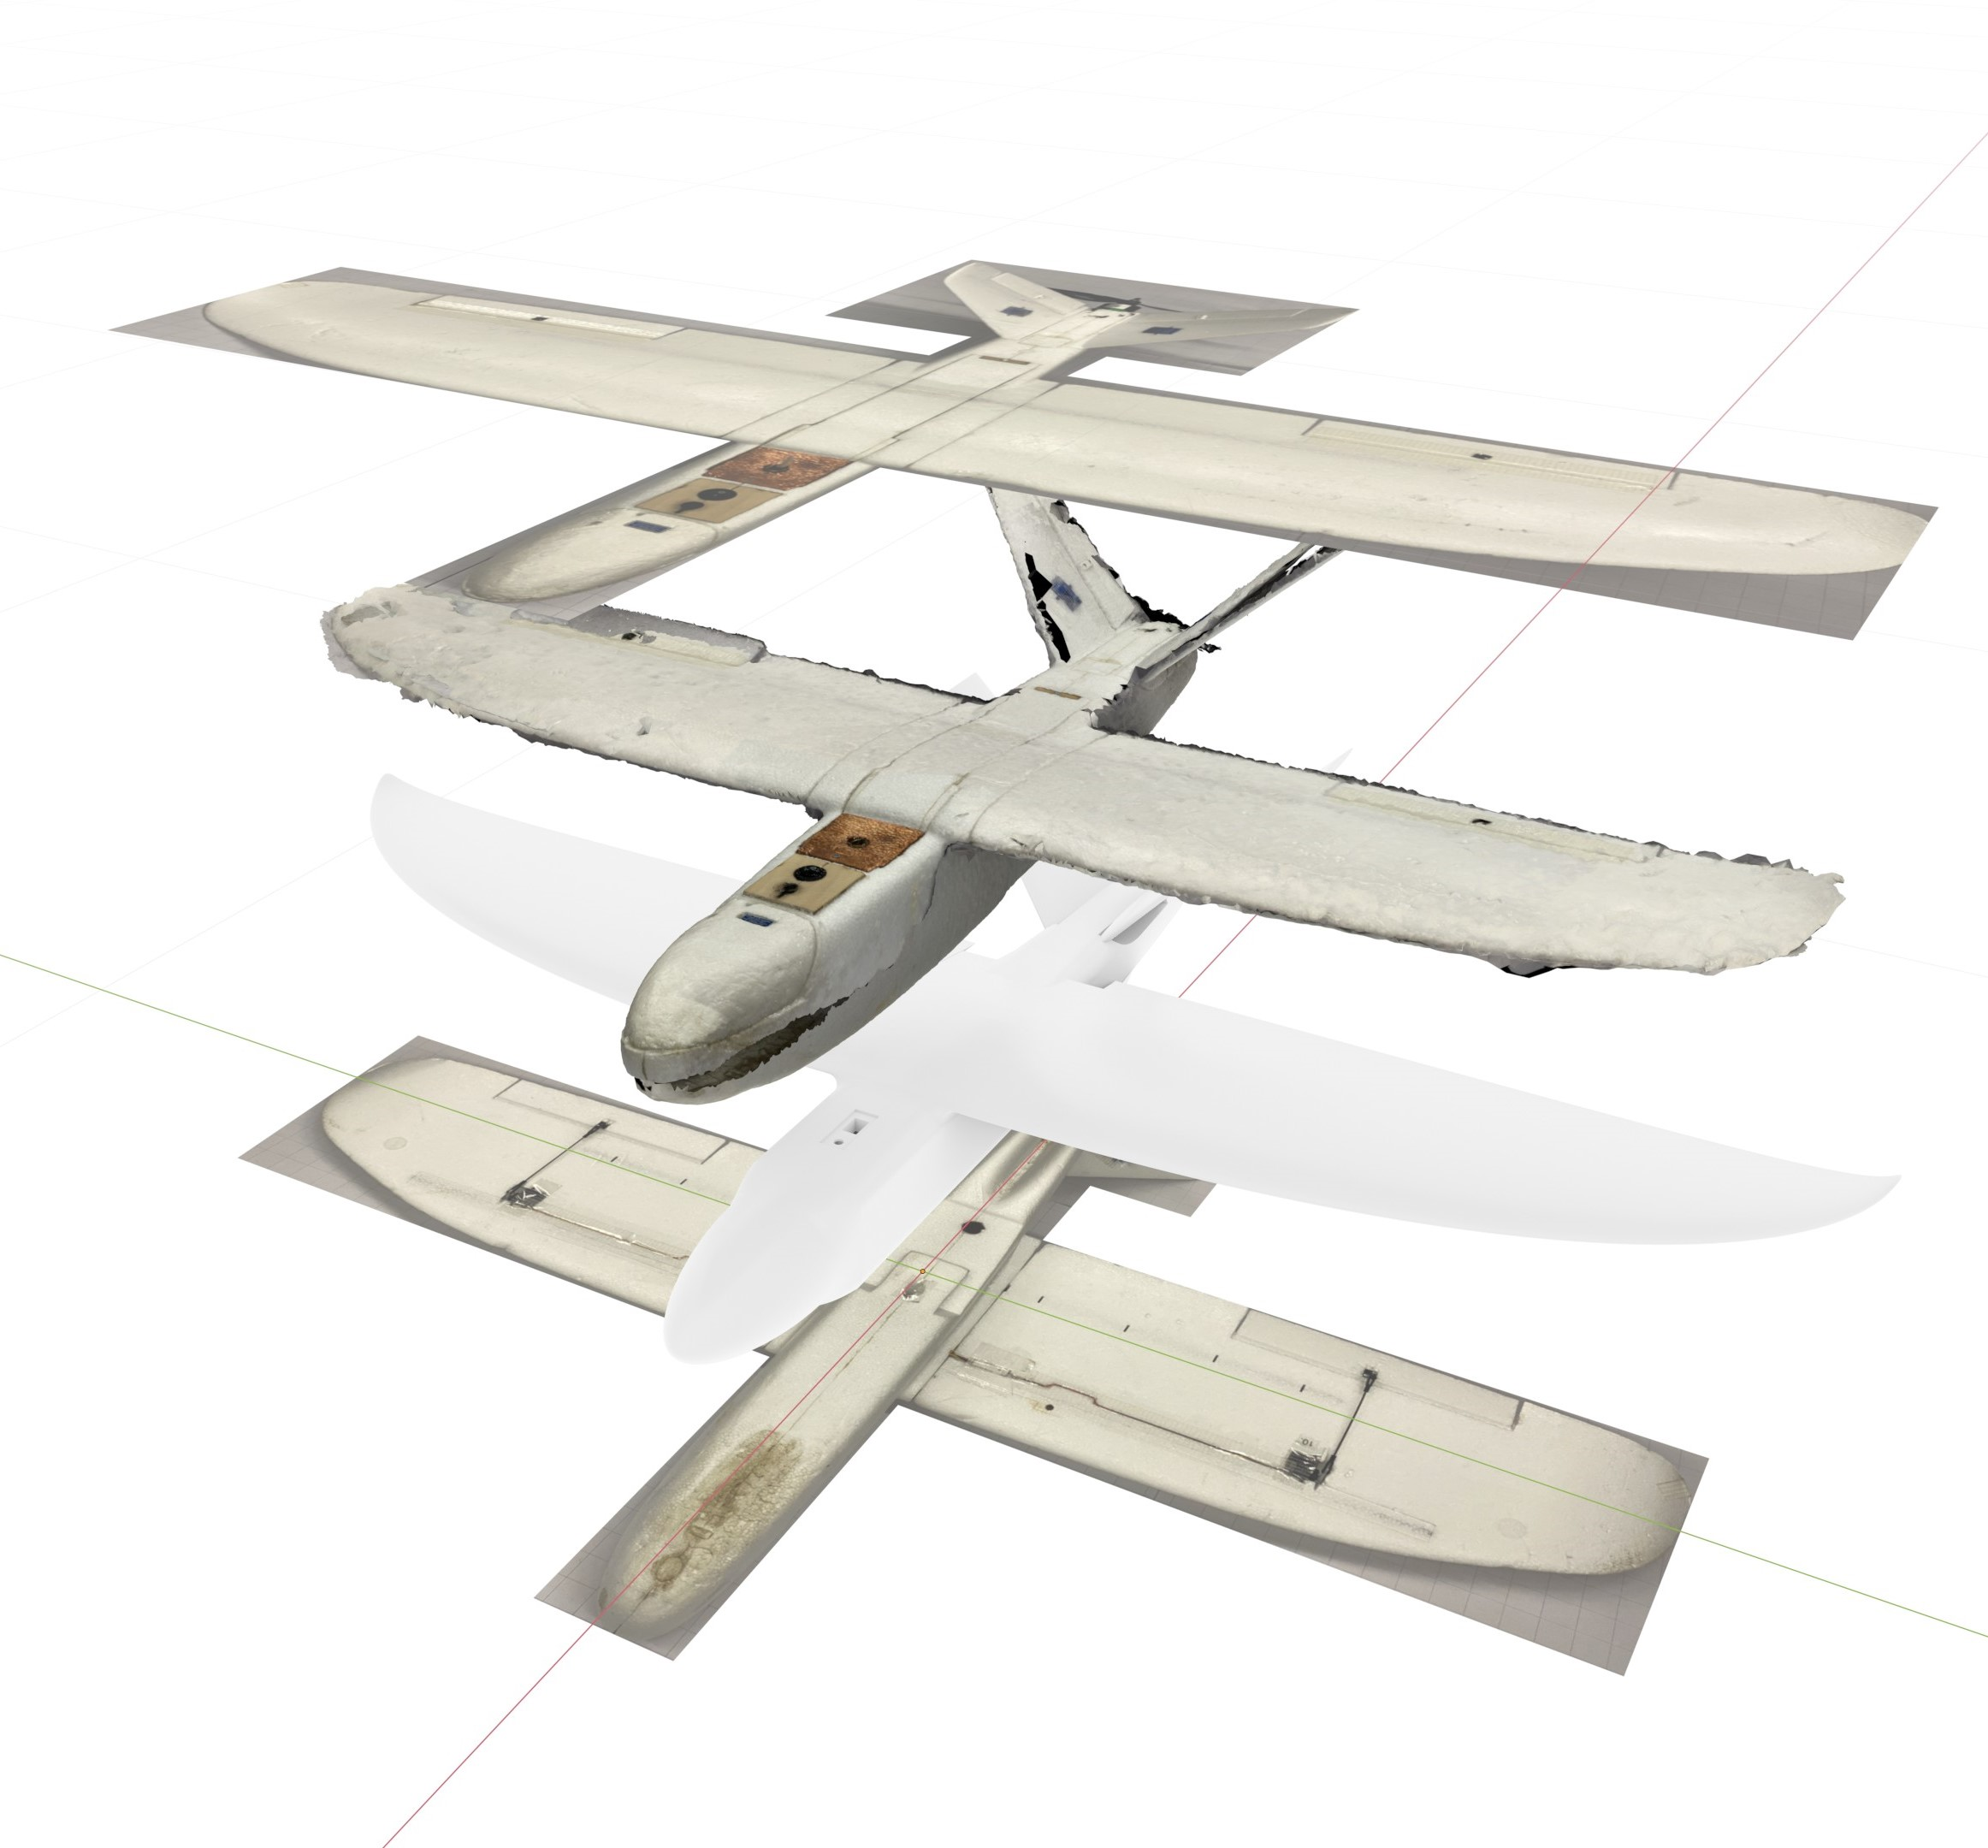
\includegraphics[width=\textwidth]{gfx/prod/plane/plane5.jpg}
\caption{Unterschiedliche Schritte der Modellierung}
\label{drohne_modell}
\end{center}
\end{figure}

\subsection{Shading}

Das aus dem CAD importierte Modell besitzt eine ungleichmäßige Topologie, weshalb ein Abwickeln nur mit viel Aufwand realisiert werden hätte können. Deswegen wurde eine prozedurale Textur für das Styropor verwendet. Diese Textur ist volumetrisch, und benötigt daher kein zweidimensional abgewickeltes Modell. Mit einem glänzenden Material und Volumenstreuung konnte der nötige Realismus erreicht werden. Unter Volumenstreuung versteht man, dass Lichtstrahlen nicht nur von der Oberfläche, sondern auch innerhalb des Objektes reflektiert werden. Das fertig Material ist in \autoref{shading} zu sehen. Das durchscheinen des Lichtes zwischen den einzelnen simulierten Styroporkugeln ist hier besonders gut sichtbar.

\begin{figure}[H]
\begin{center}
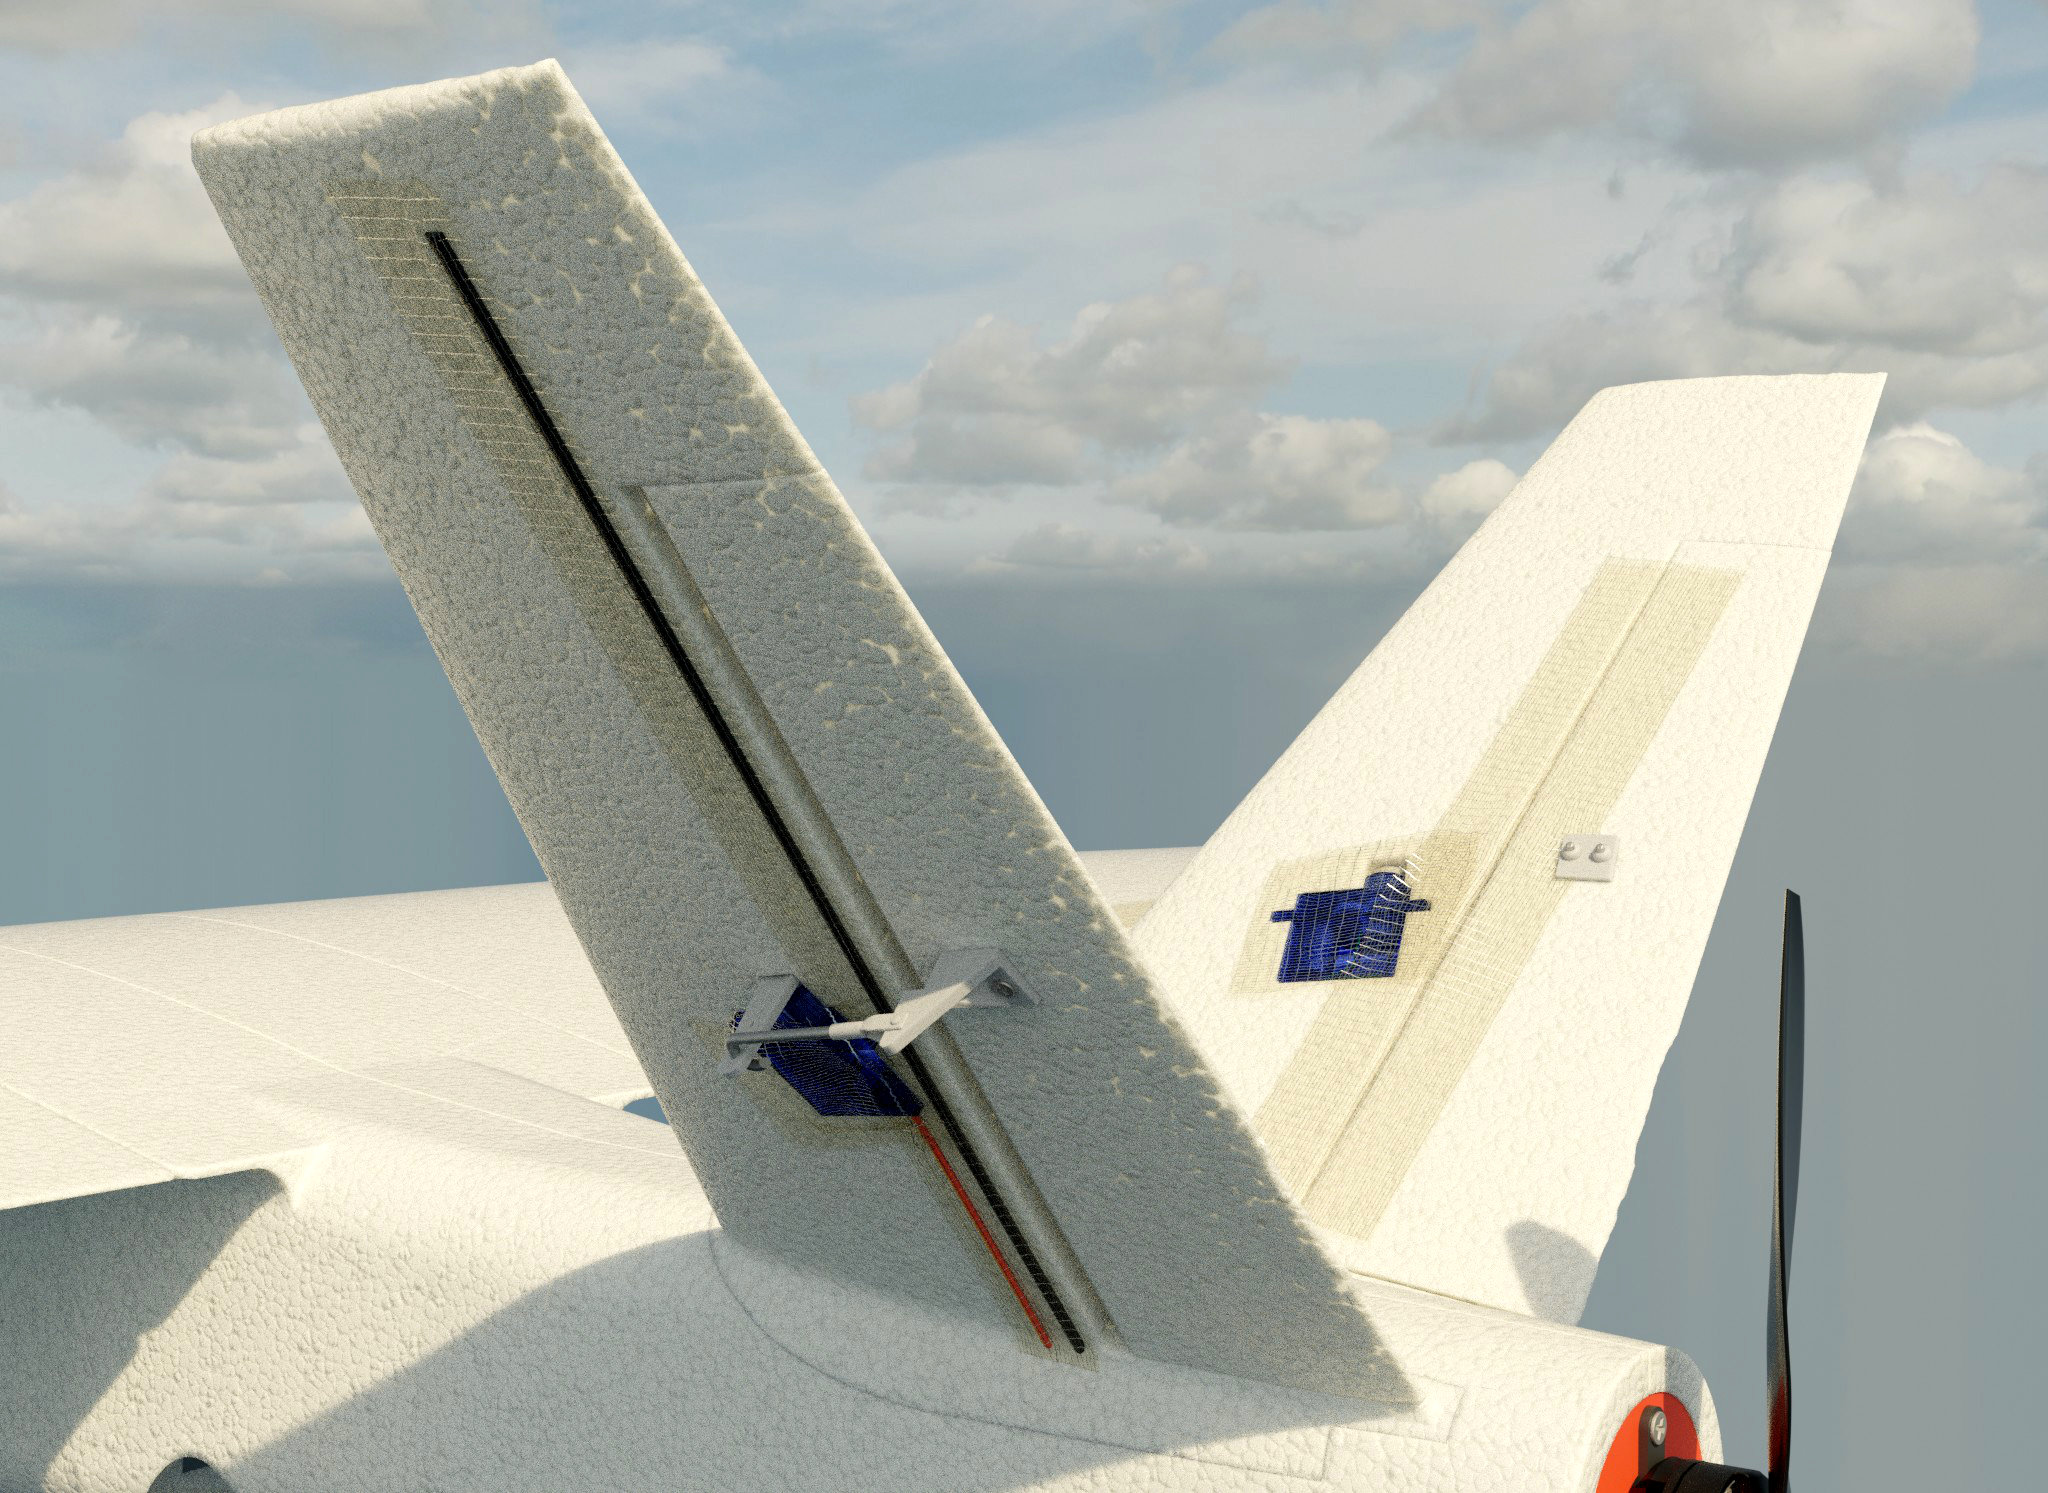
\includegraphics[width=\textwidth]{gfx/prod/plane/shading.jpg}
\caption{Nahaufnahme der fertigen Drohne}
\label{shading}
\end{center}
\end{figure}

Das Thema der später hinzugefügten Bauchbinden sollte auch im Intro aufgenommen werden. Deswegen wurde entschieden im Intro den Filmtitel (in \autoref{intro_text} zu sehen), optisch an die Bauchbinden anzugleichen (siehe \autoref{sec:bauchbinden}). Das heißt, dass im Dreidimensionalen ein Rechteck mit einem satiniertem Glas-Material und einem Titel sowie Untertitel erstellt wurde.

\begin{figure}[H]
\begin{center}

\includegraphics[width=\textwidth]{gfx/prod/env/intro_text.jpg}
\caption{Objekte für den Text im Intro}
\label{intro_text}
\end{center}
\end{figure}

\subsection{Rigging}

Unter Rigging versteht man eine Technik, bei der komplexere Bewegungen definiert werden, mithilfe von Skeletten, welche aus Knochen bestehen. Üblicherweise geschieht dies bei Charaktern, weshalb die Begriffe Skelett und Knochen geläufig sind. \footfullcite{rigging}\\
Geriggt wurden die Leitwerke der Drohne und alle Objekte, welche damit im Zusammenhang stehen. Das bedeutet die zwei Klappen an den beiden Leitwerken, sowie die Klappen an den Flügeln. Hierbei mussten die Bewegungen aller Objekte definiert werden, welche bewegen. In Reihenfolge des Effektes sind das die Servomotoren, der Hebel, die Verbindungsstange, die Befestigung am Leitwerk, das Leitwerk selber, sowie in Teilen das Klebeband.\\
Die Bewegungen wurden mit einem Skelett mit Inverser Kinematik versehen. Dies bedeutet, dass die Position des Hebels des Servomotors und die Position der Verbindungsstange errechnet werden, in Abhängigkeit der Position des Leitwerkes. Das Ziel, welches die Kinematik erreichen muss, ist mit türkiser Farbe in \autoref{rig} markiert. Die passende Deformation des Klebebandes wurde mit einem ``Weight Painting'' erstellt. Hierbei wird definiert, welcher Teil des Objektes statisch ist, und welcher Teil sich mit dem Knochen mitbewegt \footfullcite{weight_paint}.
%todo Weightpainting, Bone, Armature, (IK)

\begin{figure}[H]
\begin{center}
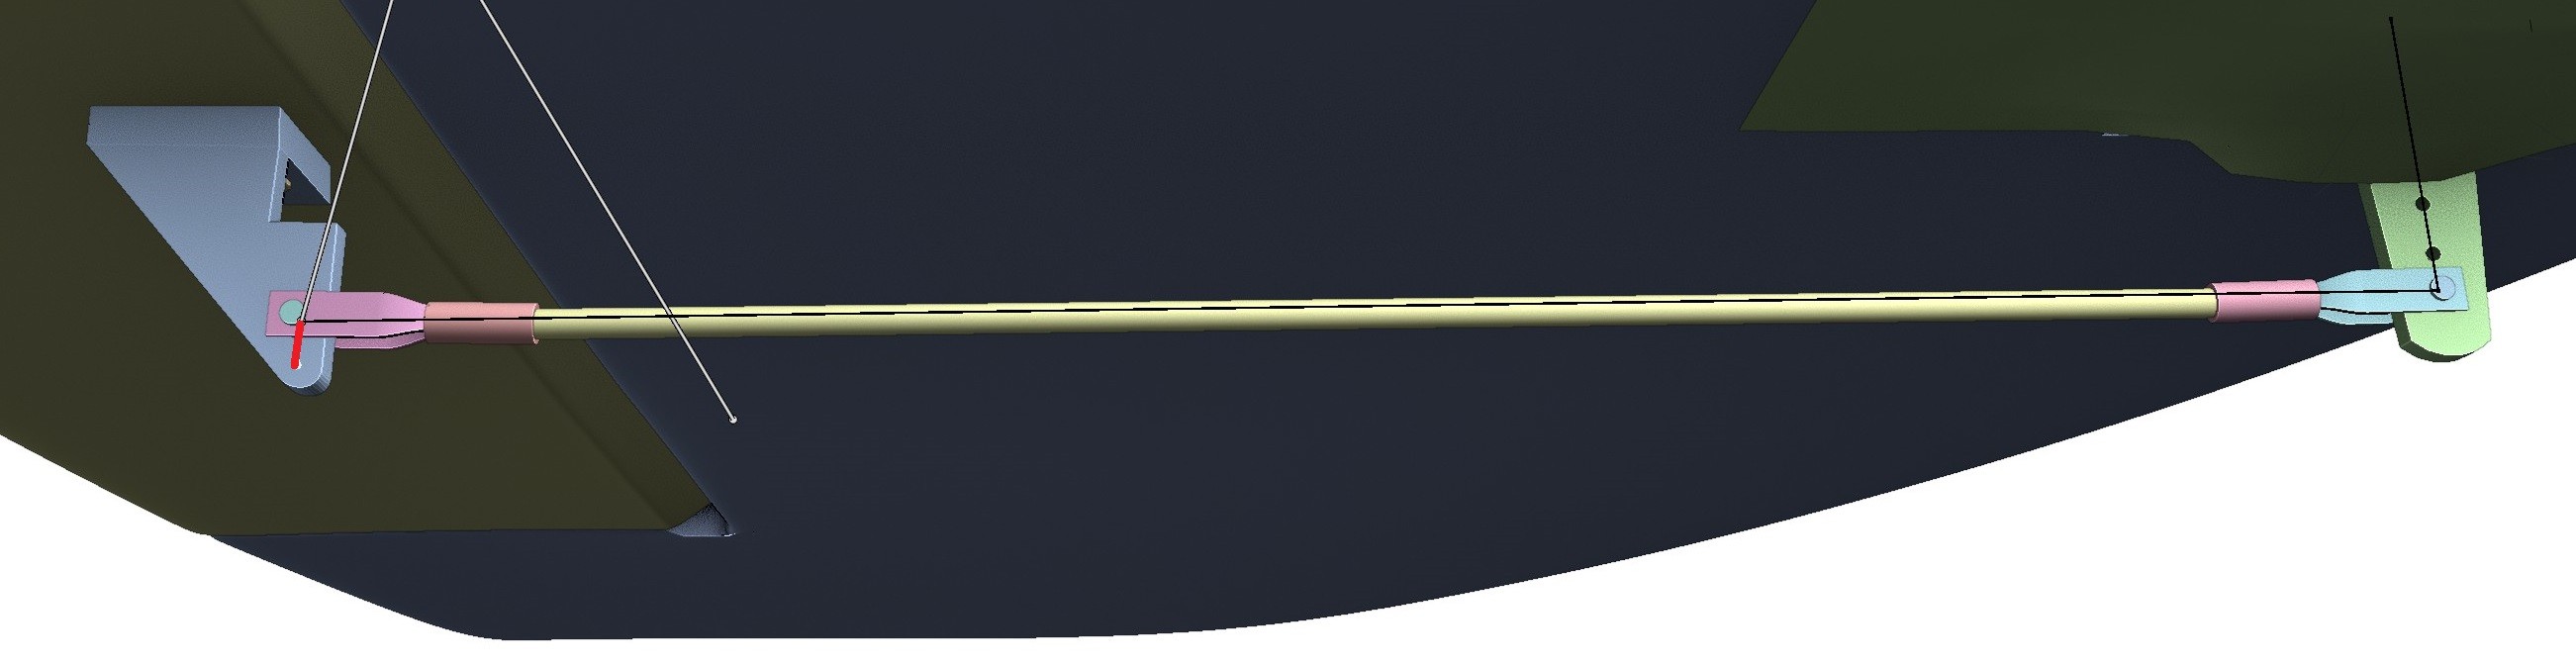
\includegraphics[width=\textwidth]{gfx/prod/plane/plane7.jpg}
\caption{Darstellung des Rigs am Beispiel der Tragfläche}
\label{rig}
\end{center}
\end{figure}

Um den Aufwand bei der Animation zu reduzieren, wurde ein Knochen in Nähe der Antenne eingefügt, welcher ähnlich einem Steuerknüppel im Flugzeug funktioniert. Somit können alle Klappen mit diesem Objekt angesteuert werden. Die Steuerung stimmt ebenfalls mit dem Prinzip des Steuerknüppels zusammen -- so muss bspw. das Objekt in Richtung der Flugrichtung geneigt werden, damit das Flugzeug sich nach unten neigt. Um dies zu erreichen dreht die Rotation des Steuerknüppels in Flugrichtung die Klappen an den Tragflächen. Die Rotation des Steuerknüppels um die beiden anderen Achsen wird an die Leitwerke gesendet. Hierbei werden die unterschiedlichen Bewegungsrichtungen aufeinander addiert. \\
Die Antenne, welche sich im Fahrtwind mitbewegt, wurde mit einem ``Bendy-Bone'' erreicht. Hierunter versteht man einen Knochen, welcher sich selber mit einem Spline-Algorithmus deformieren kann. Daher musste hier kein aufwändiges Weight-Painting erstellt werden.

\begin{figure}[H]
\begin{center}
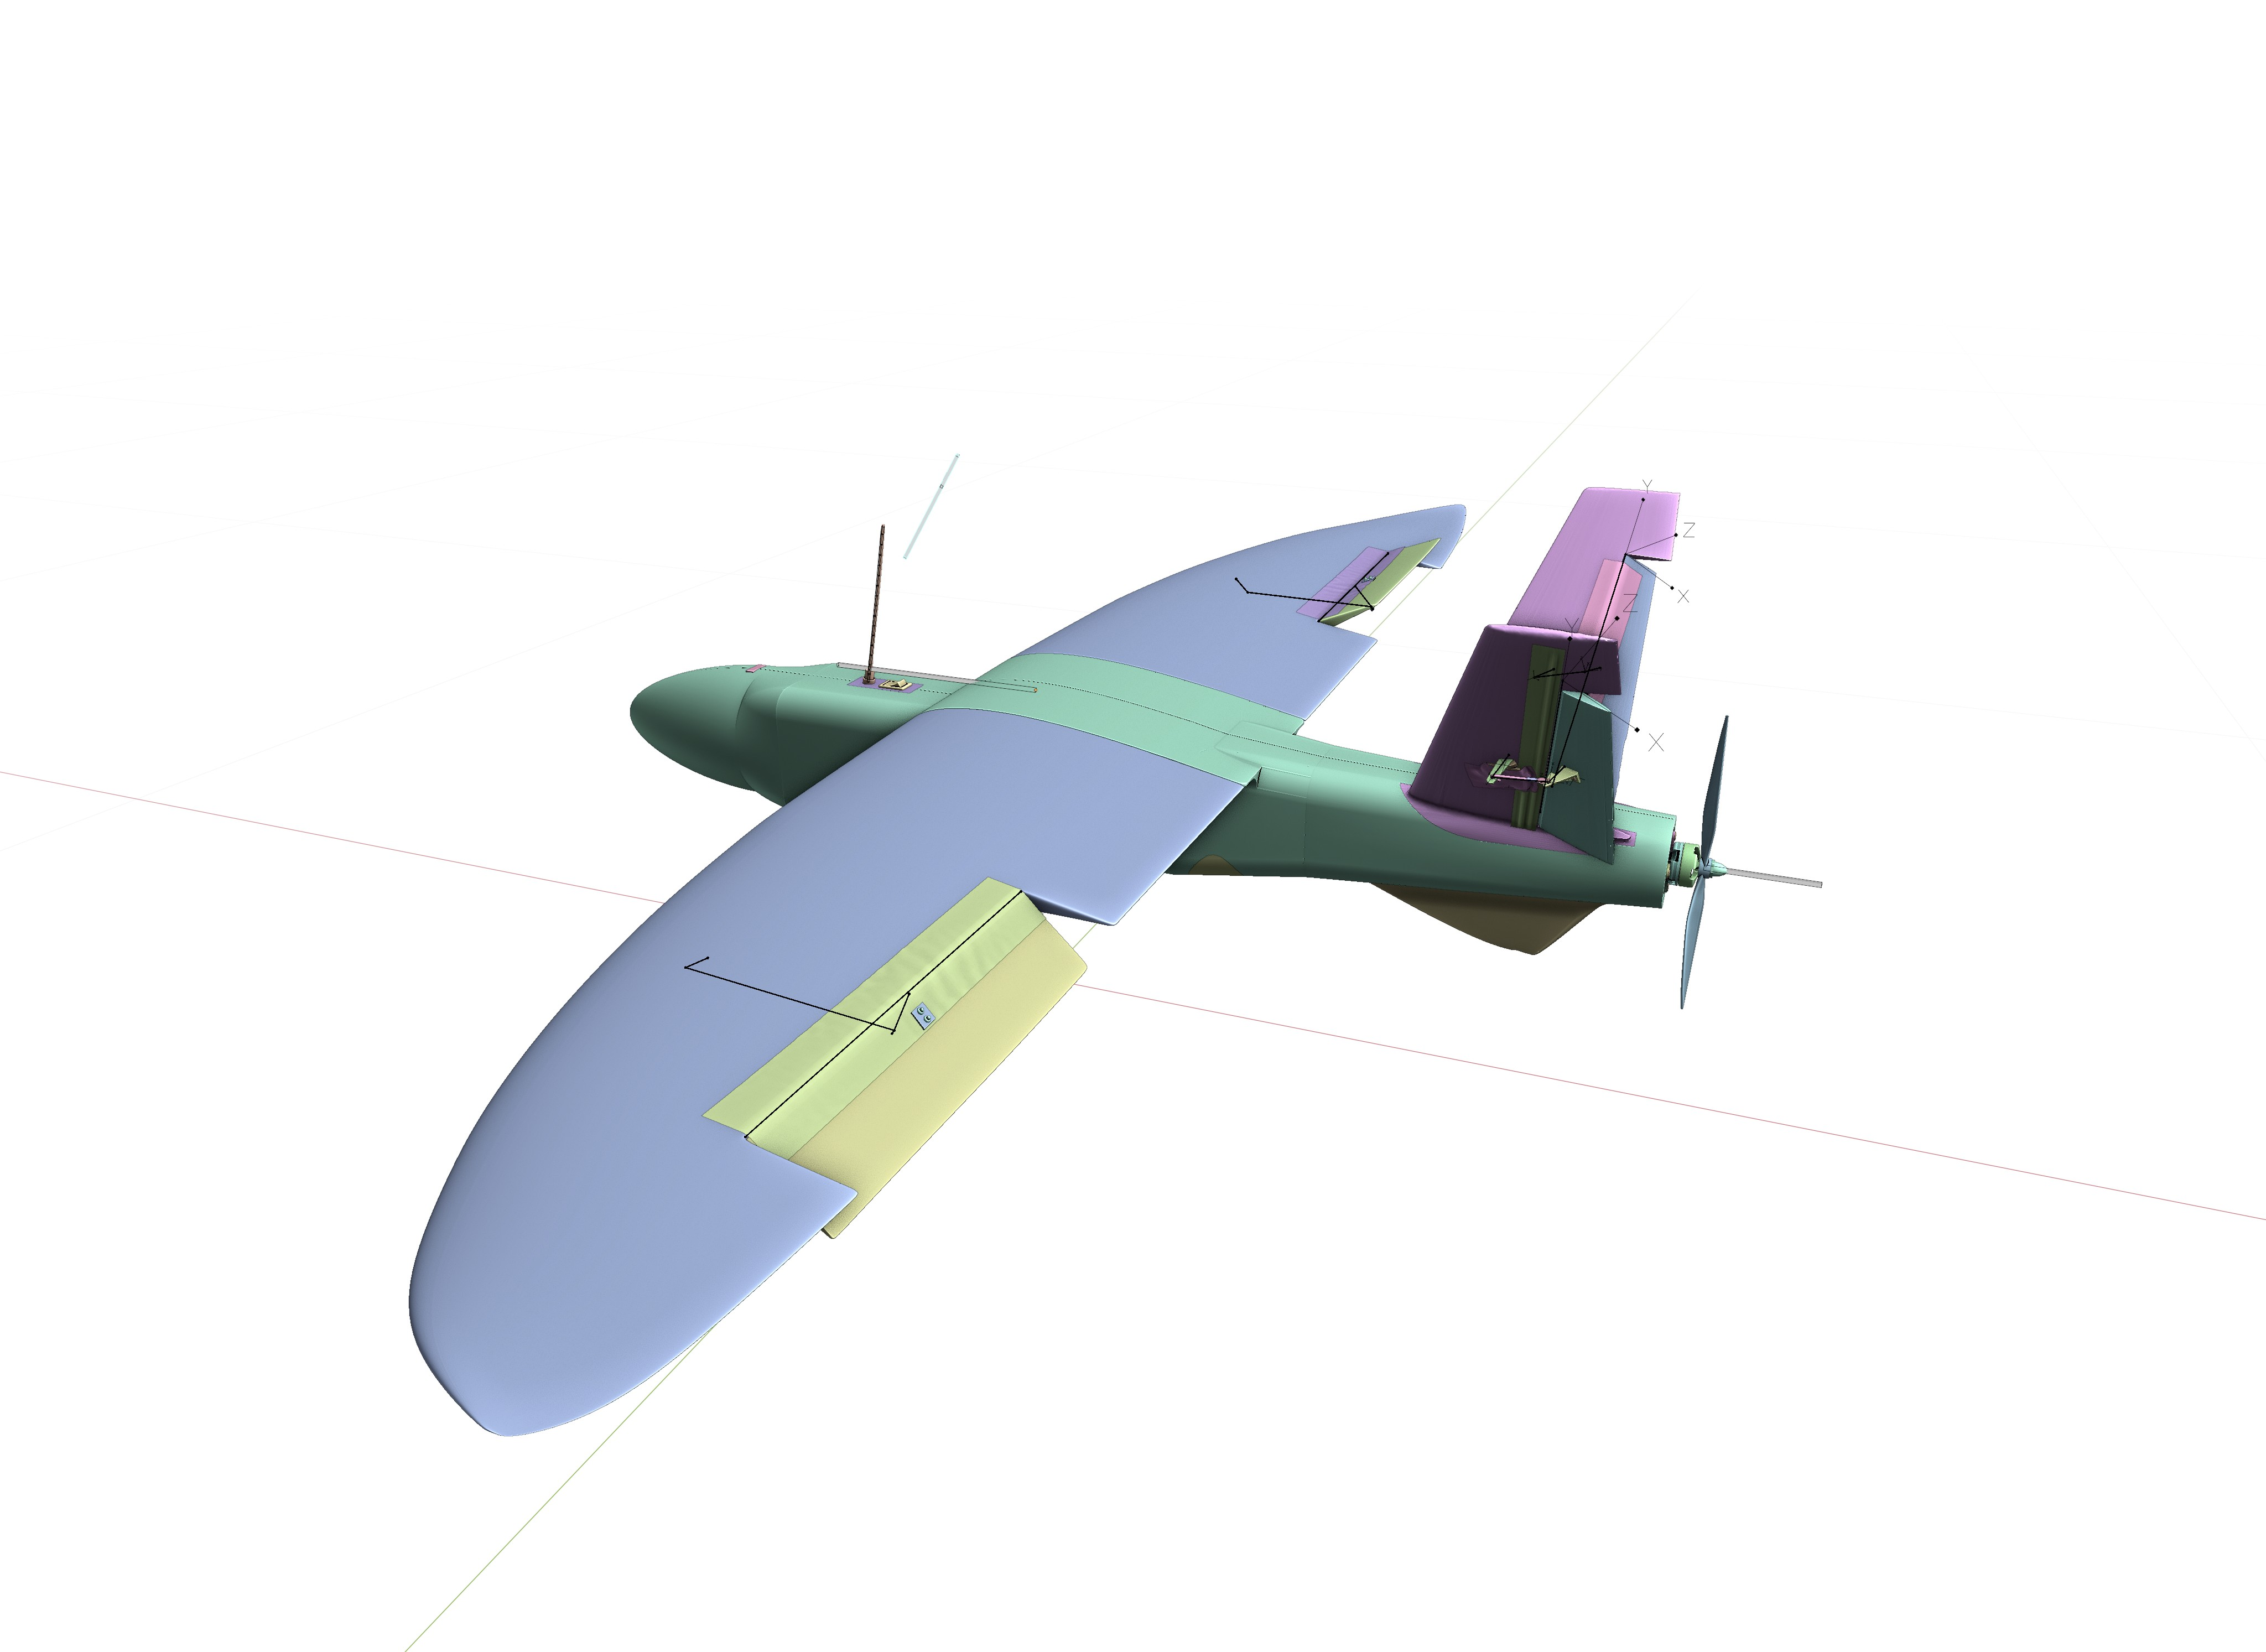
\includegraphics[width=\textwidth]{gfx/prod/plane/plane8.jpg}
\caption{Maximale Ausschläge der Leitwerke}
\label{rigged_plane}
\end{center}
\end{figure}

\section{Animation}

Die Bewegung des Flugzeuges wurde mit einem visuellen Programmiersystem in Blender erstellt (siehe \autoref{animation_nodes}). Das Prinzip dahinter ist, dass eine Kurve erstellt wird, welcher das Flugzeug folgt. Mit der Kurve selber ist die Ausrichtung und die Position der Drohne berechenbar. Weiterhin wird der Kurvenradius berechnet, wovon der Rollgrad des Flugzeuges abhängig ist. Abschließend wird in Abhängigkeit der Rotation des Flugzeuges die Stellung der Klappen berechnet.

\begin{figure}[H]
\begin{center}
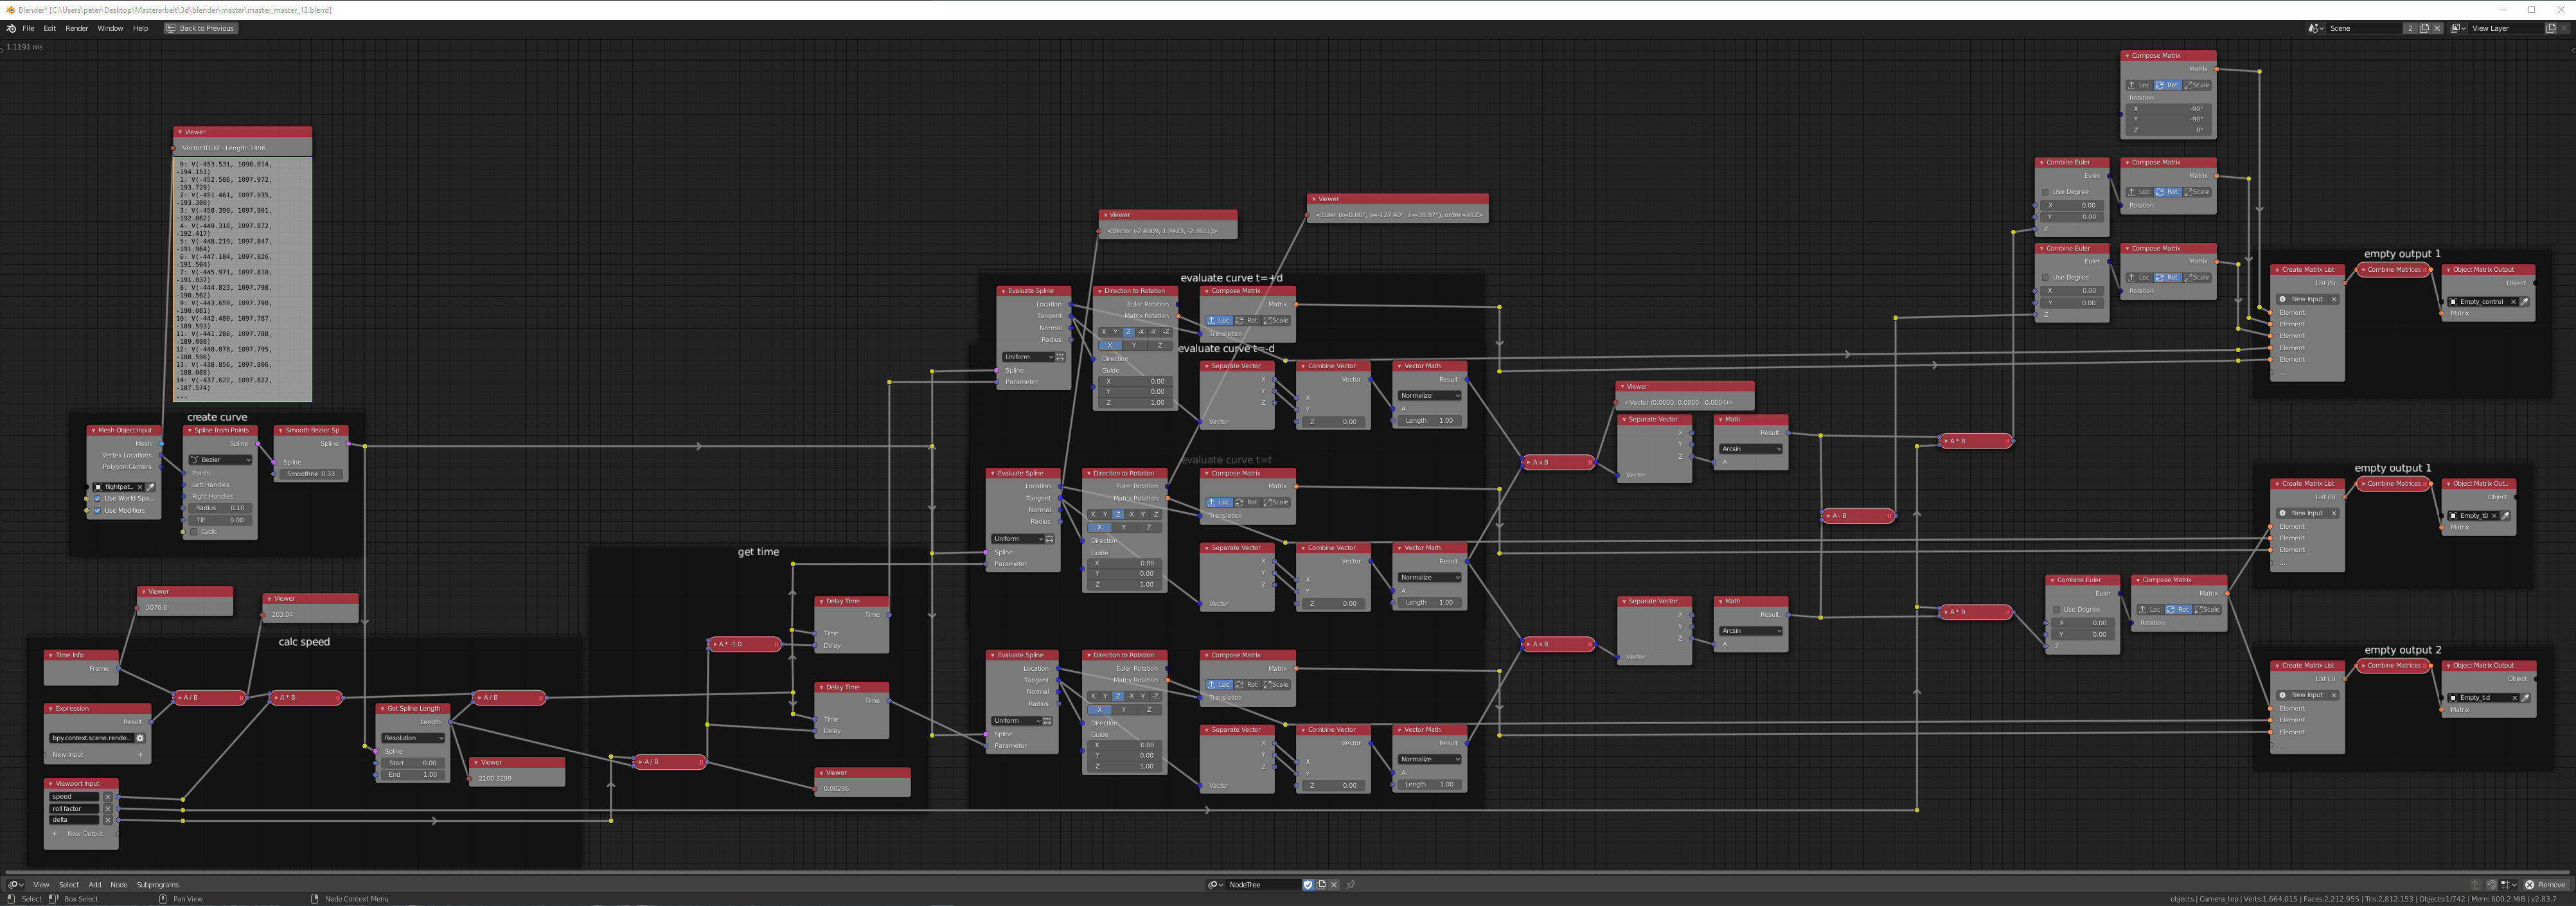
\includegraphics[width=\textwidth]{gfx/prod/plane/animation_nodes.jpg}
\caption{Übersicht über die visuelle Programmierung in Animation Nodes}
\label{animation_nodes}
\end{center}
\end{figure}

Der Kurvenradius wurde mithilfe von zwei weiteren Objekten errechnet, indem deren Rotation vor und hinter dem Flugzeug abgefragt wurde (siehe \autoref{an_flight}). Dies kann man jedoch auch als zeitlichen Versatz sehen, sodass dies einem Zeitversatz $ +\Delta $ bzw. $ -\Delta $ entspricht. Dadurch können numerische Ableitungen errechnet werden.
Als Kurve wurde keine Spline sondern eine NURBS gewählt, da diese so eingestellt werden kann, dass sie in der ersten Ableitung stetig ist. Einzige Ausnahme in der das Flugzeug nicht mit diesem System animiert wurde, ist die Landung. Hier war es einfacher das abrupte abbremsen und das nachschaukeln im Wasser, händisch nachzustellen.
%todo Quelle
Der Kamera wurde mit einem Child-Of-Constraint die Eigenschaft gegeben, dass die Position von der des Flugzeuges abhängig ist. Zusätzlich wurde der Kamera eine Bewegung über Keyframes gegeben, damit sie sich um die Drohne herumbewegen kann. Somit war ein einfacher Workflow für die Kameraanimation vorhanden und die Kameraanimation musste nicht nachbearbeitet werden, wenn der Flugpfad geändert wurde.\\
Der in \autoref{sec:konzept:outline} angesprochene Realismus bezieht sich grundsätzlich auch auf Animationen. Im Flug wurde eine realistische Bewegung als nicht wichtig eingestuft, weil in Film und Fernsehen nur große Flugzeuge gezeigt werden, welche sich während dem Flug sehr ruhig bewegen. Daher wurde hier auf starke Bewegungen aufgrund von bspw. Turbulenzen verzichtet. Bei der Landung hingegen wurde das Schaukeln des Bootes und der Kamera wieder aufgegriffen, und ein möglichst gutes Eingliedern in den restlichen Film zu ermöglichen.

\begin{figure}[H]
\begin{center}
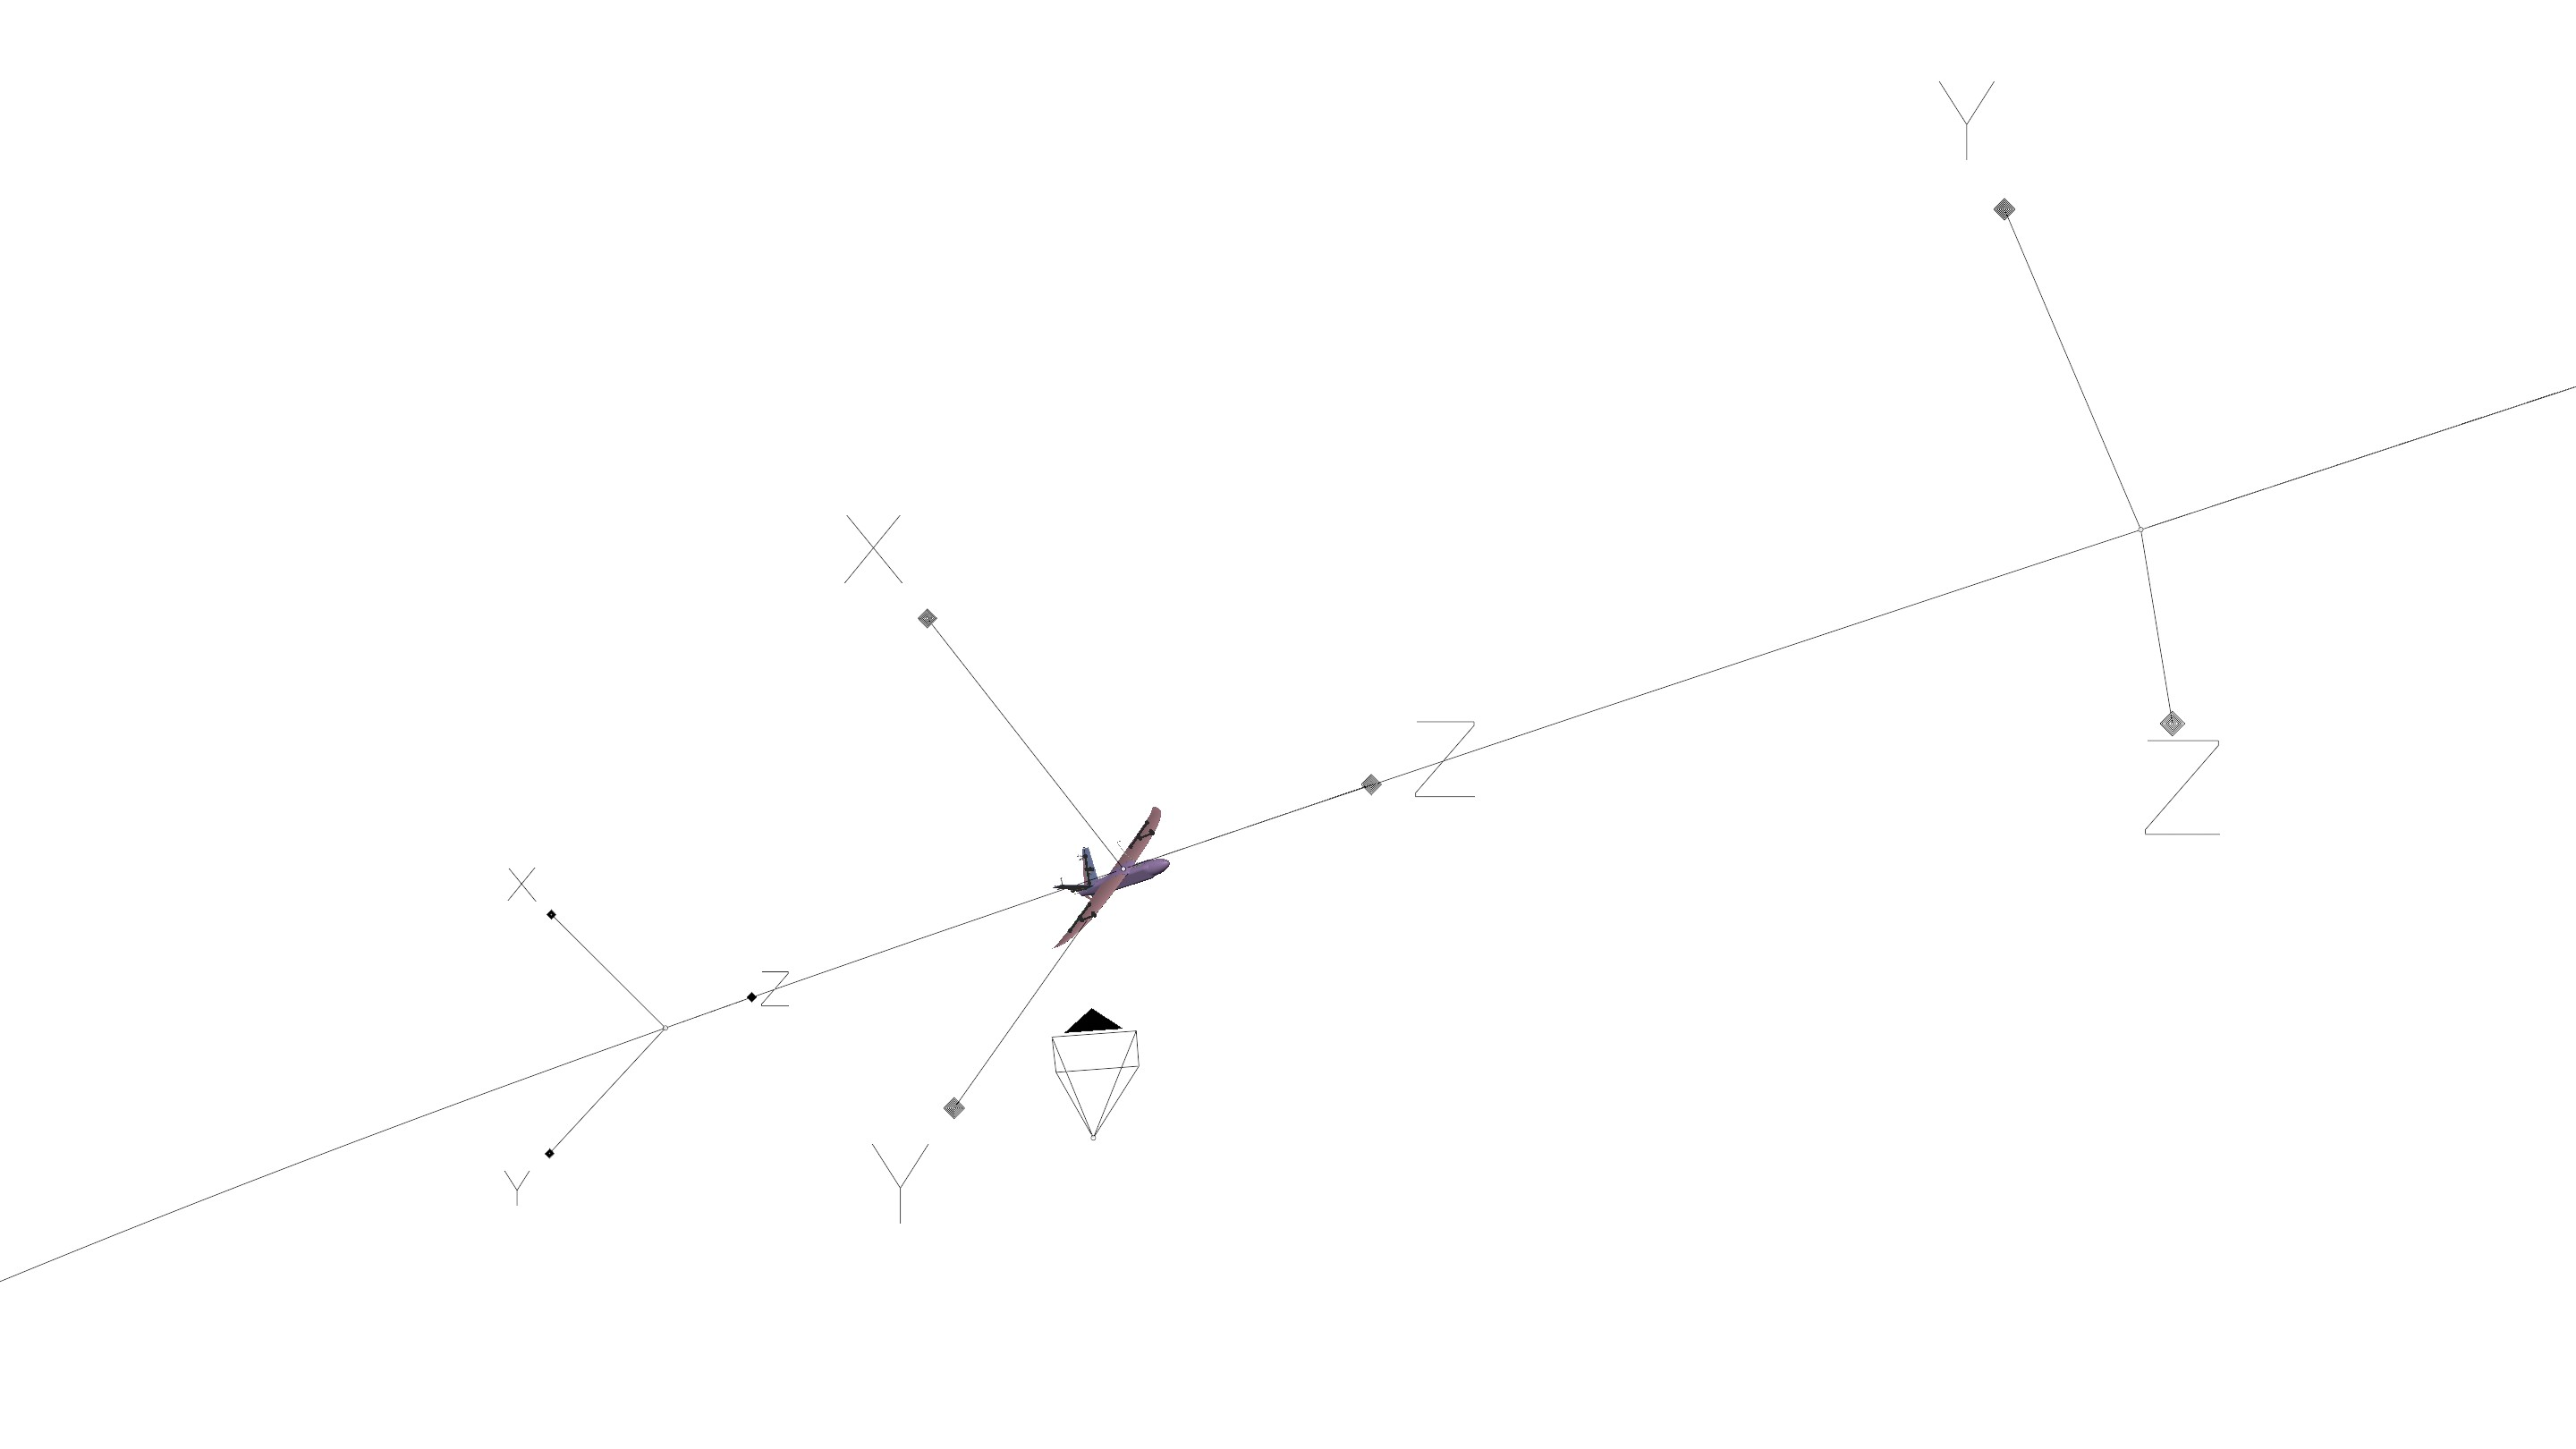
\includegraphics[width=\textwidth]{gfx/prod/plane/an_flight.jpg}
\caption{Drohne mit Flugpfad und Rotationsabfragen}
\label{an_flight}
\end{center}
\end{figure}

Die Darstellung der Landung ist einer der sechs wichtigen Funktionen der Drohne, die in diesem Film enthalten sein sollen.
Da jedoch kein Videomaterial von der Landung vorhanden war, musste diese virtuell nachgebaut werden. Hierzu wurde, wie oben beschrieben, die Drohne animiert. Weiterhin wurden Partikel -- kleine Kugeln mit Wassermaterial -- in der Umgebung der Drohne in die Luft geschleudert. Mit etwa 150.000 Partikel konnte der Effekt der Wasserspritzer erzielt werden (siehe \autoref{particles}).

\begin{figure}[H]
\begin{center}
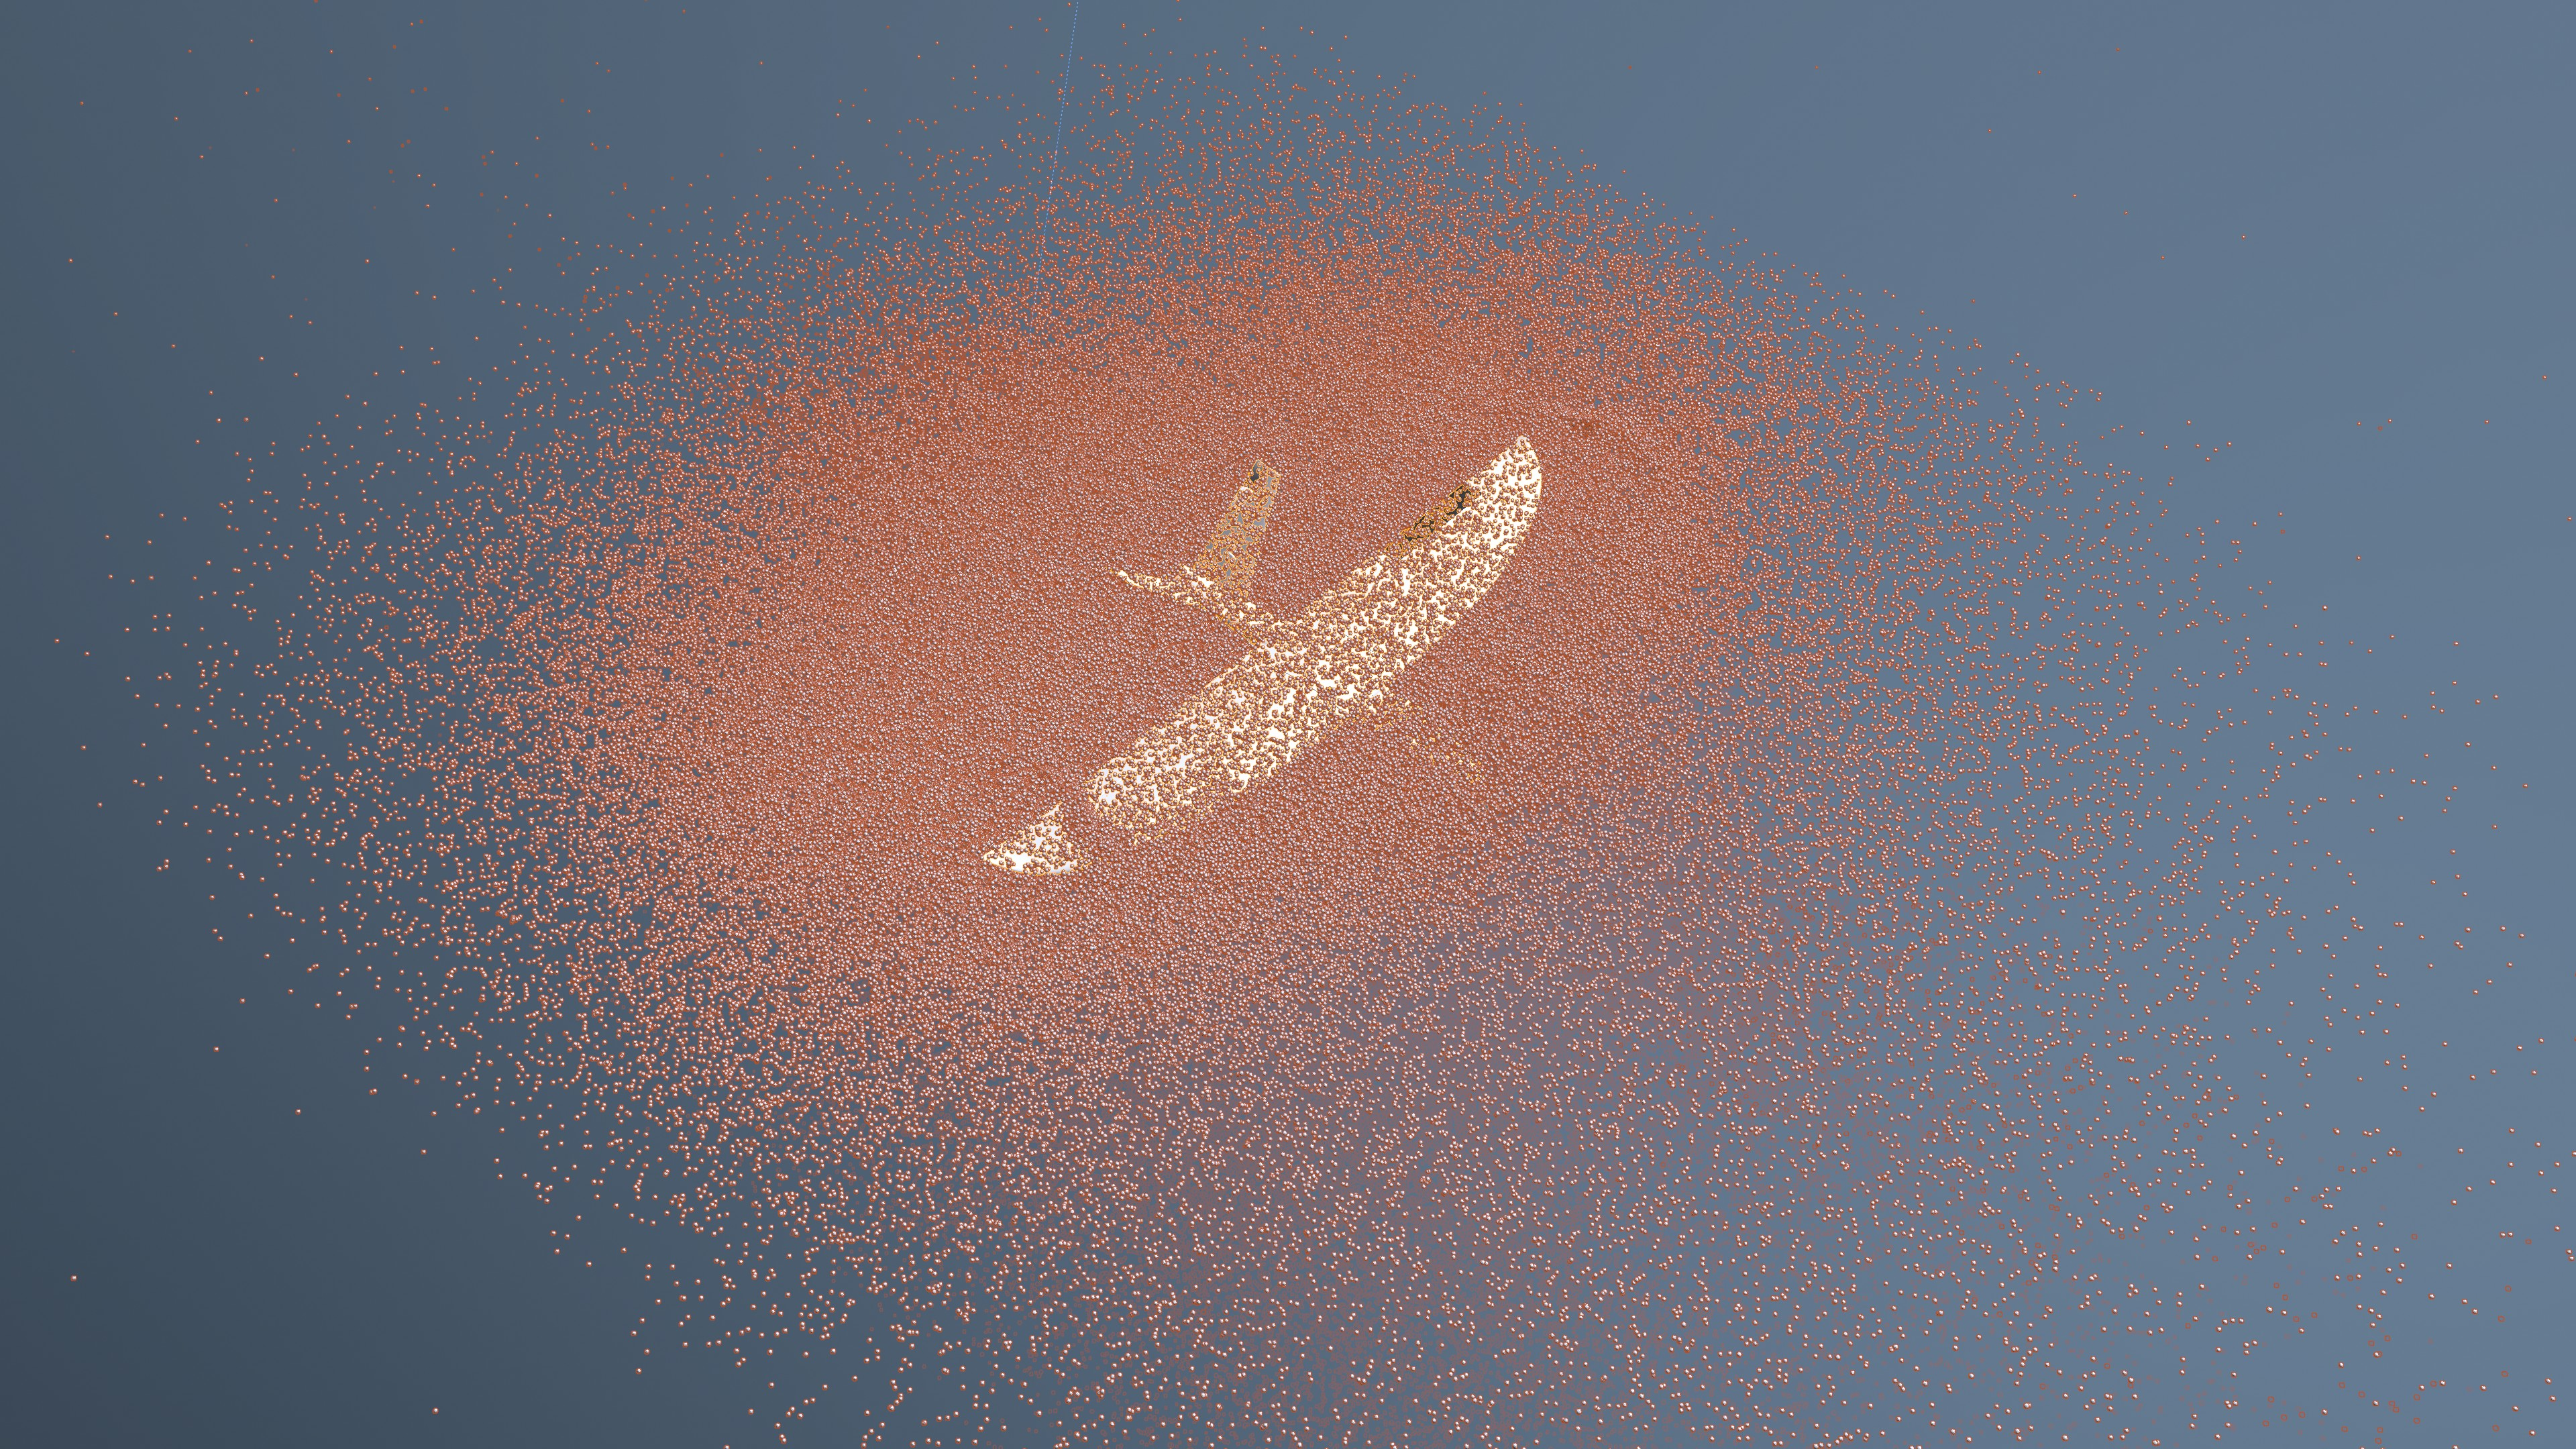
\includegraphics[width=\textwidth]{gfx/prod/plane/particles.jpg}
\caption{Wasserpartikel in der Umgebung der Drohne}
\label{particles}
\end{center}
\end{figure}


\section{Rendering}

Das nun fertiggestellte und animierte Modell wurde nun gerendert. Hierunter versteht man dass in Abhängigkeit der Lichtquellen -- in diesem Fall des Himmels -- Licht und Schattenwurf des Modells berechnet wird. Um einen möglichst realistischen Look zu erreichen, wurde entschieden mit dem Path-Tracer ``Cycles'' zu arbeiten. Dieser verwendet einen sehr rechenaufwändigen stochastischen Algorithmus. Dies bedeutet, dass mit vielen Proben getestet wird, wie sich Photonen in der Szene verhalten würden. Mit steigender Anzahl der Proben reduziert sich die Streuung, weswegen das Bildrauschen reduziert wird. \footfullcite{cycles}\\
Für dieses Projekt stand nur ein Standrechner mit einer handelsüblichen Grafikkarte zur Verfügung, weshalb nur 512 Proben pro Pixel berechnet wurden. Das sichtbare Rauschen wurde dann mit einem Filter entfernt. In \autoref{denoising} ist der Unterschied zwischen Rohmaterial (linke Bildhälfte) und gefiltertem Bild (rechte Bildhälfte) zu sehen. Insgesamt belief sich damit die Rechenzeit bei 1550 Bildern und bei 100 Sekunden pro Bild auf etwa 48 Stunden.

\begin{figure}[H]
\begin{center}
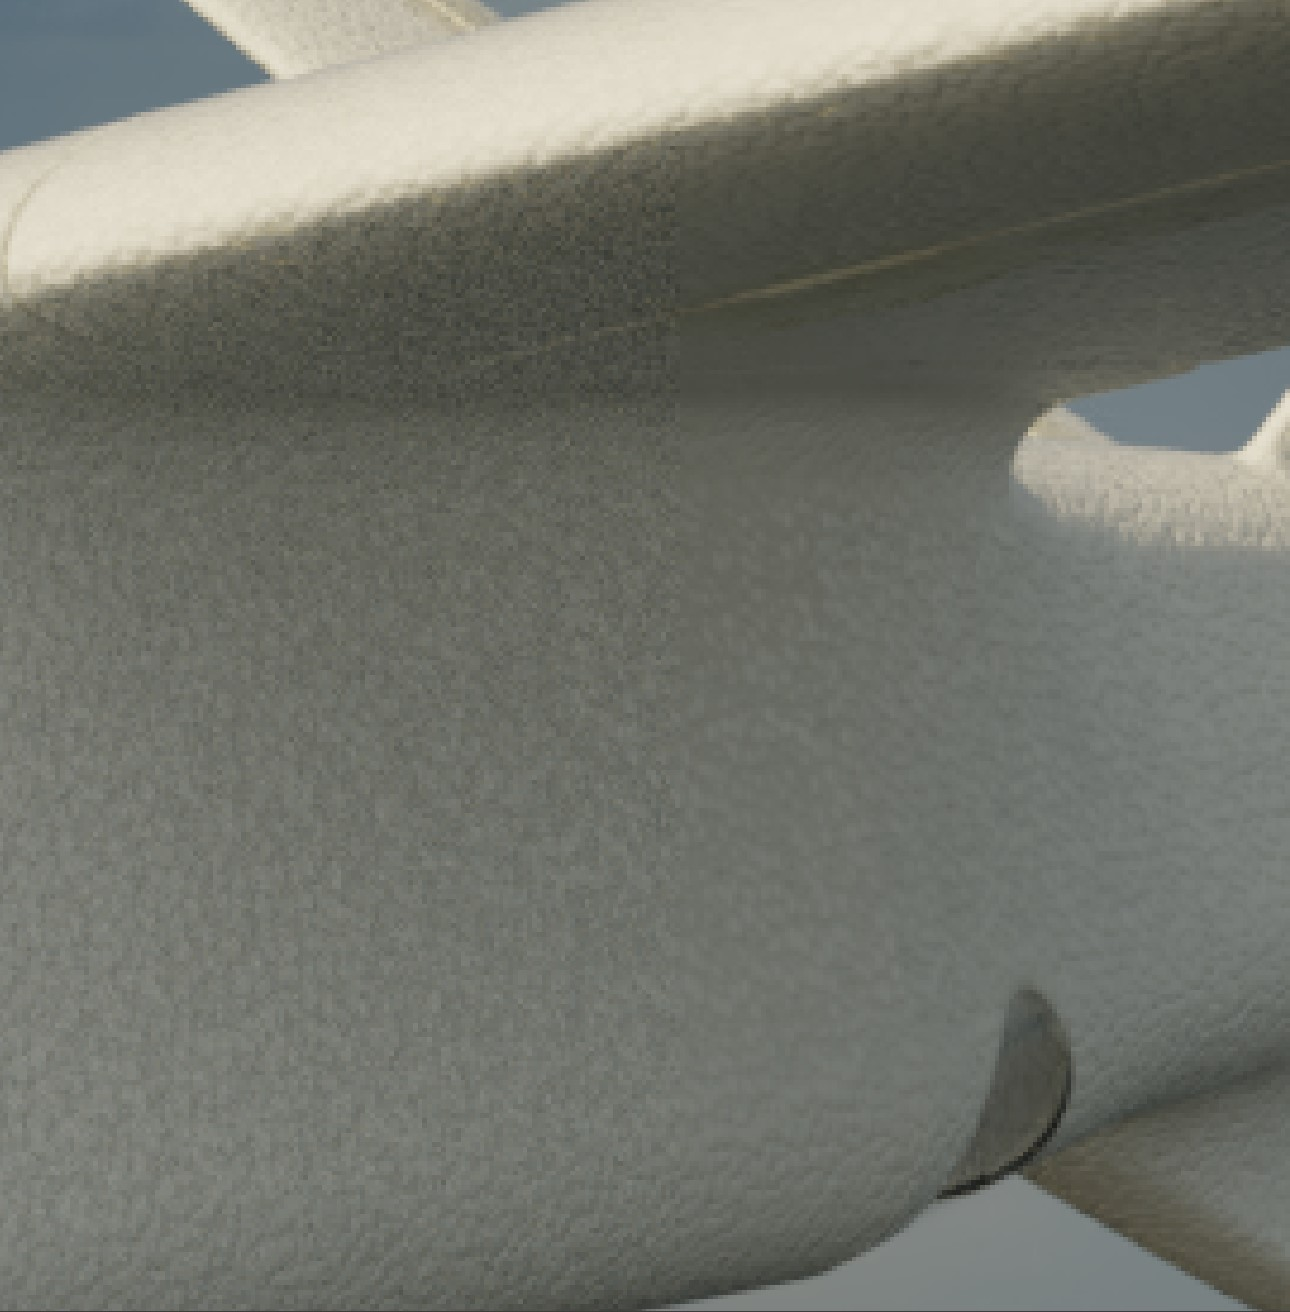
\includegraphics[width=\textwidth]{gfx/post/denoising.jpg}
\caption{Unterschied zwischen Augsangsbild und rauschgefilertem Bild}
\label{denoising}
\end{center}
\end{figure}

Für diesen Vorgang und für die Möglichkeit bei der Nachbearbeitung den vollen Farbumfang zu Verfügung zu haben, wurden die Bilder als openEXR exportiert. Dies hatte den Nachteil, dass pro gerendertem Bild etwa 120 mB Speicherplatz zur Verfügung stehen mussten. Zählt man unterschiedliche Iterationen dazu, mussten etwa 600 GB Speicherplatz zur Verfügung stehen.\\
Eine Herausforderung beim Rendern der Szene waren die unterschiedlichen Größenverhältnisse. Die kleine Drohne musste im Kontext mit dem weitläufigen Meer dargestellt werden. Daher kam die Rendereengine mit ihrer einfachen Gleitkommazahl an Genauigkeit an ihre Grenzen. Dies hatte Artefakte zur Folge, die in \autoref{bug} zu sehen sind. Diese entstehen, weil durch die fehlende Genauigkeit nicht entschieden werden kann, ob ein Polygon vor oder hinter dem anderen liegt.

\begin{figure}[H]
\begin{center}
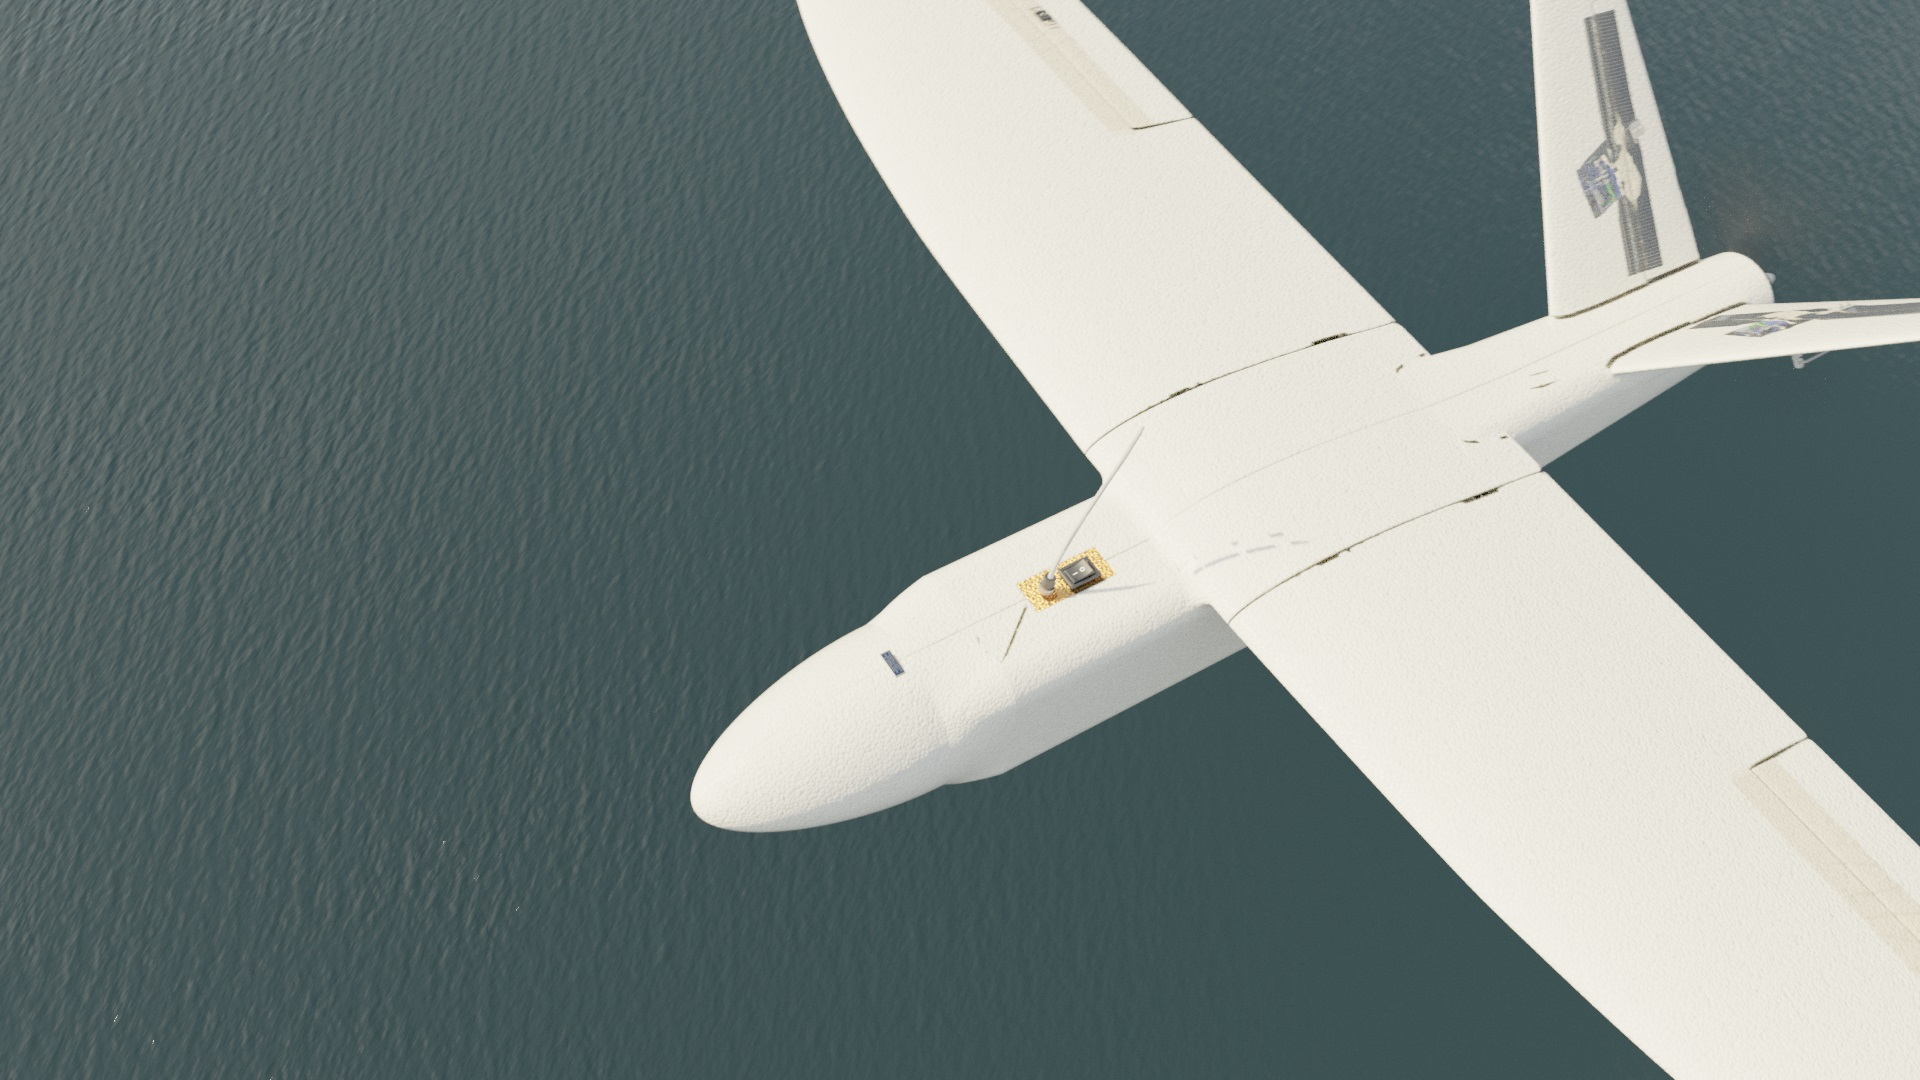
\includegraphics[width=\textwidth]{gfx/prod/plane/bug.jpg}
\caption{Artefakte an der Drohne}
\label{bug}
\end{center}
\end{figure}


Um dies zu umgehen, wurde die gesamte Szene so verschoben, dass die Drohne immer möglichste nahe am Ursprung ist. In \autoref{transform} ist sichtbar, dass der Flugpfad zunächst unterhalb des Ursprunges (Kreuzung von roter und grüner Linie) ist, und in der zweiten Abbildung ist der Flugpfad oberhalb des Ursprunges.

\begin{figure}[H]
\begin{tabular}{cc}
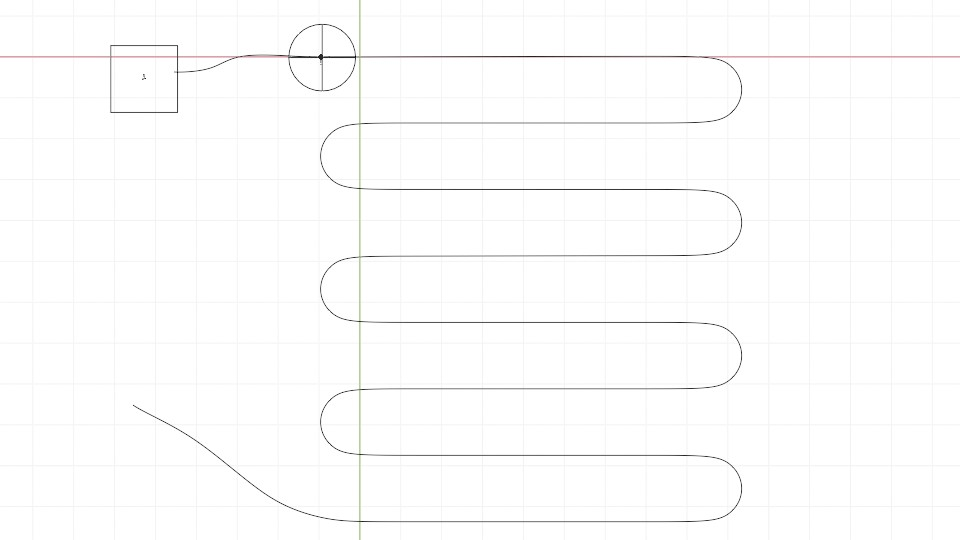
\includegraphics[width=0.5\textwidth]{gfx/prod/plane/flightpath1.jpg}&
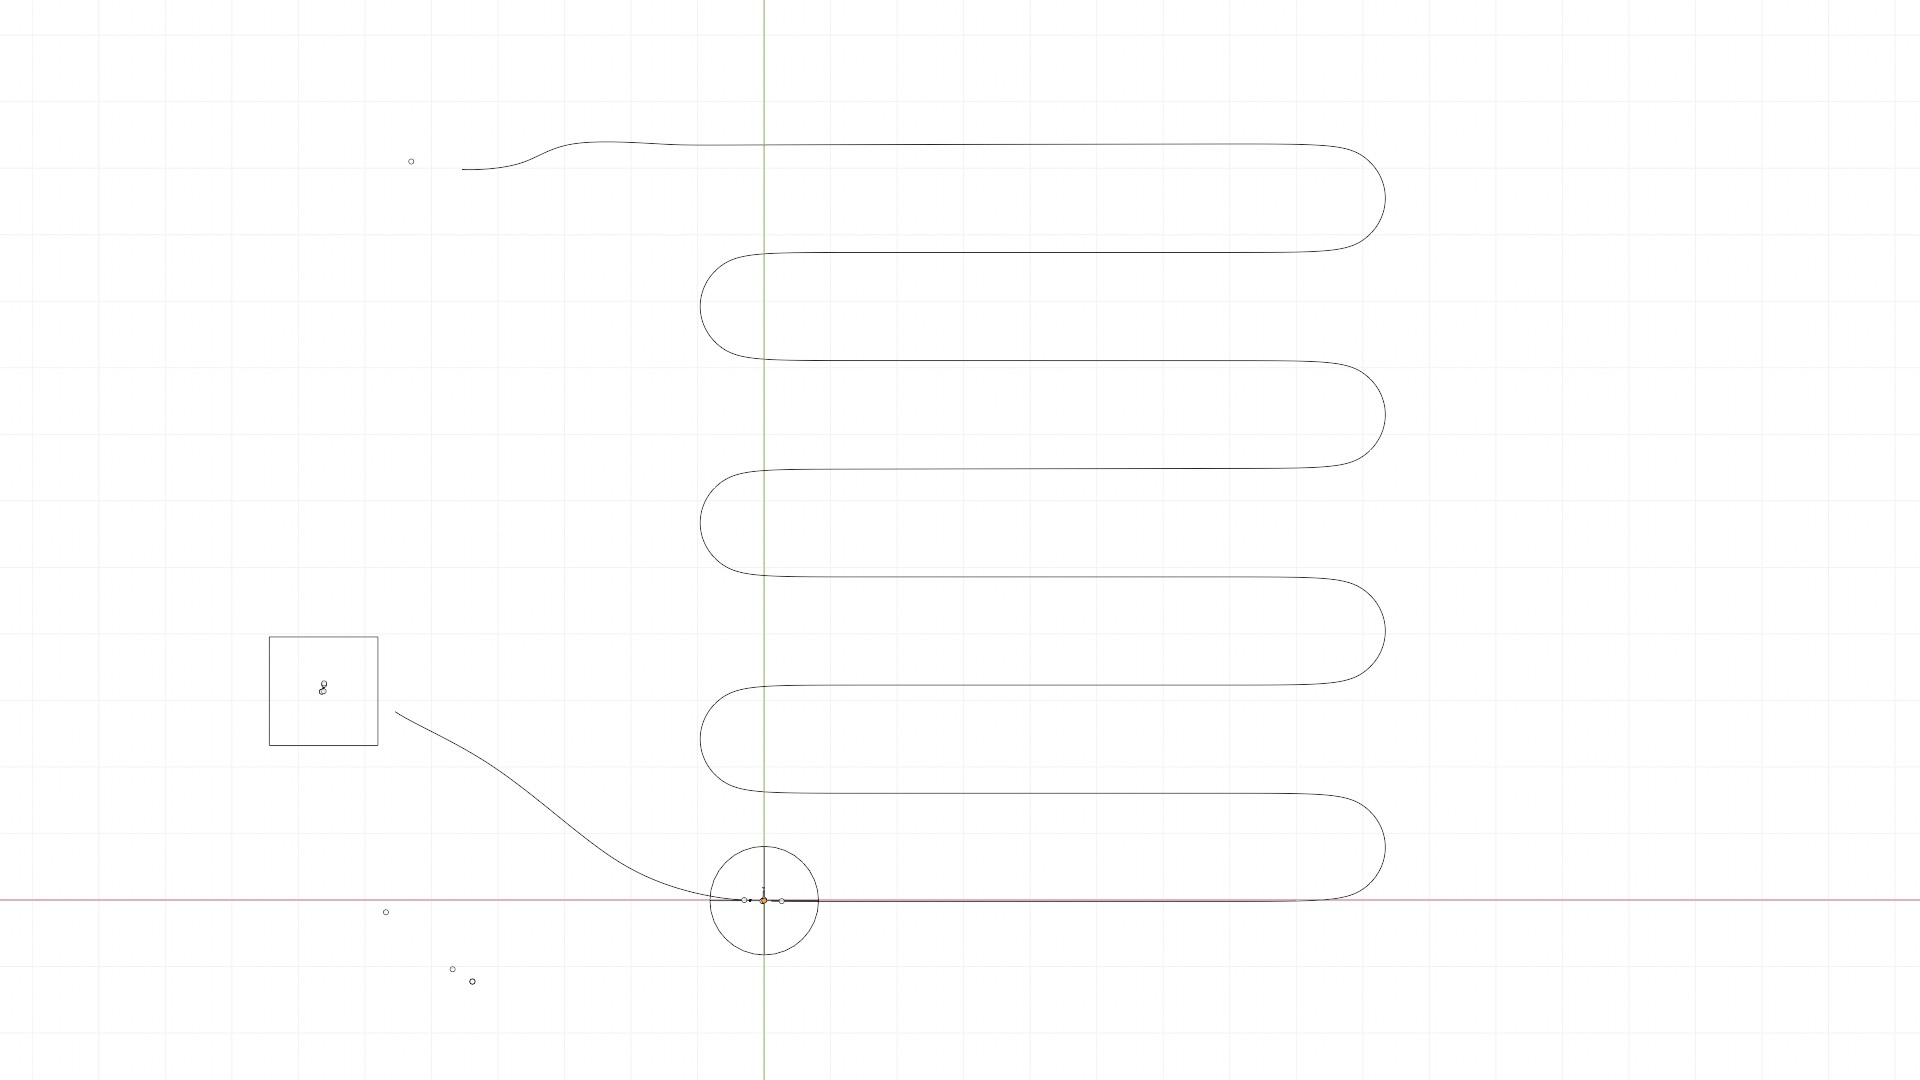
\includegraphics[width=0.5\textwidth]{gfx/prod/plane/flightpath2.jpg}
\end{tabular}
\caption{Verschiebung der Szene}
\label{transform}
\end{figure}